\documentclass[12pt]{article}
\usepackage{latexsym}
\usepackage{amsfonts}
\usepackage{amsmath}
\usepackage{xspace}
\usepackage{tikz}
\usepackage{tikz-3dplot}
\usepackage{graphicx}
\usepackage{pst-solides3d}
\usepackage[utf8]{inputenc}
\usetikzlibrary{calc}
\usepackage{amssymb}
\usepackage{natbib}
\usepackage{pgfplots}
\pgfplotsset{width=15cm,compat=1.9}


%%Formatting
\topmargin -.2in
\textheight 9.2in
\evensidemargin 0in
\oddsidemargin 0in
\textwidth 6.5in
\parskip .1in

\pagestyle{empty}

\begin{document}

\hrule
\vspace{.2cm}

{\Large \noindent Math 112 Honors
\hfill
B\'ela Bajnok}

\vspace{.3cm}
\hrule

{\Large \noindent 
Final Exam
\hfill
Fall 2020}

\vspace{.3cm}
\hrule

\noindent NAME:  Quan Nguyen

\noindent \hrulefill\rule{0pt}{4pt}

\noindent Write and sign the full Honor Pledge here:

\vspace{2mm}

I affirm that I have upheld the highest principles of honesty and integrity in my academic work and have not witnessed a violation of the Honor Code. \par

Quan Nguyen

\vspace{8mm}

\noindent \hrulefill\rule{0pt}{4pt}

\noindent {\bf General instructions -- Please read!}

\begin{itemize}
  
\item The purpose of this exam is to give you an opportunity to explore a series of complex and challenging questions, gain a comprehensive view of calculus and its applications, and develop some creative writing, problem solving, and research skills.

\item  {\bf All your assertions must be completely and fully justified.} At the same time, you should aim to be as concise as possible; avoid overly lengthy arguments and unnecessary components.  Your grade will be based on both mathematical accuracy and clarity of presentation.

\item 
Your finished exam should  {\bf stand alone as an article}, consisting of complete sentences, thorough explanations, and exhibit correct grammar and punctuation.

\item I encourage you to prepare your exam using LaTeX.  However, you may use instead other typesetting programs that you like, and you may use hand-writing or hand-drawing for some parts of your exam.  In any case, {\bf the final version that you submit must be in PDF format.}  

\item It is acceptable (and even encouraged) to discuss the exams with other students in your class or with the PLA.  However,  {\bf  you must individually write up all parts of your exams.}  To elaborate:

\begin{itemize}  
\item	You are absolutely allowed to discuss every aspect of the exams, starting with the mathematics involved and up to the details of the technical issues of typesetting.
\item	You are allowed to meet with another student and show parts of your work during the discussion.
\item	You are NOT allowed to send parts of your work to another student.
\item	You are absolutely NOT allowed to have other students copy your work.
\item	You are absolutely NOT allowed to copy another students work.
\end{itemize}


\item {\bf You may use the text, your notes, and your homework, but no other sources.}
 
\item You must write out a complete, honest, and detailed acknowledgment of all assistance you received and all resources you used (including other people) on all written work submitted for a grade.

\item Submit your exam to me by email at bbajnok@gettysburg.edu by the deadline announced in class.







\end{itemize}

\noindent {\bf Good luck!}


\newpage


\section{Introduction}


\noindent What is Calculus about?  

\noindent What are the main concepts and topics of Calculus 2?

\section{Six Themes of Calculus}

\subsection{Mathematical Survivor} 



\vspace*{.2in}

\noindent This game begins with $n$ people on an island.  The people are numbered 1 through $n$.  Each day, the remaining islanders vote on whether the remaining islander with the highest number can stay on the island.  If half or more of them say the person with the highest number must leave, then that person leaves the island and the game continues.  Otherwise, the game ends and the remaining islanders split a million dollars equally.  Assume the islanders act independently, are perfectly rational, and will vote in whatever way will give them the most money at the end.  How long will the game last and how many people will remain on the island at the end?


\begin{enumerate}
  
\item Work out the details of the game for small values of $n$, such as $n=1, 2, 3, \dots, 10$.  In each case, determine how long the game lasts and the number of people left on the island at the end.

\item Suppose that $n=100$.  Determine how long the game lasts and the number of people left on the island at the end.

\item Answer the questions for a general $n$.  Give your answers as functions of $n$.

\item Verify that your general answer agrees with your answers for small values of $n$ that you determined earlier. 


\end{enumerate}

\subsection{Sum(o) Wrestling} 



\vspace*{.2in}


\noindent In this problem we use Riemann sums to prove that $$\int_{a}^b x^k \; \mathrm{d}x = \frac{1}{k+1}(b^{k+1}-a^{k+1})$$ holds for $k=1$, $k=2$, and $k=3$.

\begin{enumerate}

\item Use Riemann sums to prove that $$\int_{a}^b x \; \mathrm{d}x = \frac{1}{2}(b^{2}-a^{2}).$$

\item Use Riemann sums to prove that $$\int_{a}^b x^2 \; \mathrm{d}x = \frac{1}{3}(b^{3}-a^{3}).$$

\item Use Riemann sums to prove that $$\int_{a}^b x^3 \; \mathrm{d}x = \frac{1}{4}(b^{4}-a^{4}).$$

\end{enumerate}



\subsection{Different Viewpoints} 



\vspace*{.2in}


\noindent  
A three-dimensional object is given with the following views: its front view is a square, its side view is a triangle, and its top view is a circle.

1.  Describe the object precisely in terms of its cross sections with respect to a particular direction.  (This is a standard question during job interviews at certain companies such as Microsoft.)  Note that there are two different objects with the given views---describe both.

2.  Find the volume of both objects in terms of the radius of the top view circle.





\subsection{Probability -- Prove Your Ability} 



\vspace*{.2in}


\noindent  A certain university mathematics department offers, among others, a course on Combinatorics, a course on Probability, and a course on Statistics.  On a certain day, exams are given in each class, with a maximum possible score of 10 points in each; while in Combinatorics and Probability the achievable scores were all integers, in Statistics all values between 0 and 10 were possible.  The instructors gather the following information:

\begin{itemize}
  \item In the Combinatorics class, the scores were as follows:
  
$$1, 3, 4, 5, 5, 6, 6, 6, 7, 7, 7, 7, 7, 8, 8, 8, 8, 9, 9, 10.$$

\item In the Probability class, for each integer value of $n$ between 0 and 10, inclusive, the number of students who scored $n$ points was $(15n-n^2)/2$.

\item In the Statistics class, the number of students earning $x$ points (with $x$ between 0 and 10) could be approximated by the formula

$$63 \cdot \mathrm{e}^{-(x-7)^2/4}.$$

\end{itemize}

Answer the following questions for each of the three classes.  Use histograms, Riemann sums, or definite integrals as you see fit.


\begin{enumerate}

\item  How many students scored a 7?

\item  How many students scored a 7 or higher?

\item  How many students took the exam?

\item  What was the mode (the ``most frequent'' score)?

\item  What is the probability that a ``randomly'' selected student scored a 7 or higher?

\item  What was the mean (the ``average'' score)?

\item  What was the median (the ``middle'' score)?


\end{enumerate}



\subsection{Solitaire Army} 



\vspace*{.2in}


\noindent  The game Solitaire Army is a particular version of Peg Solitaire; it was discovered by the British mathematician John Conway in 1961.   Peg Solitaire is played on a board that has holes arranged in a rectangular grid-like fashion (like squares on an infinite chess-board).  Each hole can hold one peg.  A move consists of a jump by one peg over another peg which is next to it horizontally or vertically (but not diagonally); the peg jumped over will then be removed from the board.  Each move therefore reduces the total number of pegs by one.

In the game Solitaire Army, the board is an infinite plane where one horizontal line is distinguished; it's called the demarcation line.  At the start of the game, all pegs are on one side of the demarcation line.  

1.  Verify that it is possible to send one peg forward 1, 2, 3, or 4 holes into the other side of the demarcation line.  

2.  Use geometric series to prove that it is impossible to get to further than that.  



\subsection{Some Serious Series} 



\vspace*{.2in}

Let us define the sequence $${\displaystyle (a_n)_{n=1}^{\infty} = \left(\frac{1}{10},-\frac{\pi^2}{100},+\frac{\pi^4}{1000},-\frac{\pi^6}{10000},+- \cdots \right)}$$ and the function $${\displaystyle f(x)=\frac{1}{10+x^2}}.$$

\begin{enumerate}
  
\item  

\begin{enumerate}

\item Find an explicit formula for $a_n$.  (Make sure that $a_1=1/10$.)




\item Find $\lim_{n \rightarrow \infty} a_n$.



\item Find the exact value of $\sum_{n=1}^{\infty} a_n$.



\end{enumerate}


\item  

\begin{enumerate}

\item Use a known series to find the infinite Maclaurin series $P_{\infty}(x)$ for $f(x)$.



\item Verify your answer to part (a) by finding the quartic (degree four) Maclaurin polynomial $P_{4}(x)$ for $f(x)$ using differentiation.

\item How is this problem related to Problem 1 above?


\end{enumerate}

\item  


\begin{enumerate}

\item Use integration rules to find ${\displaystyle \int f(x) \mathrm{d} x}.$

\item Use Problem 2 above to find ${\displaystyle \int f(x) \mathrm{d} x}.$


\item Use part (a) above to find the exact value of ${\displaystyle \int_0^{\pi} f(x) \mathrm{d} x}.$

\item Use part (b) above to approximate ${\displaystyle \int_0^{\pi} f(x) \mathrm{d} x}.$  Compare your answer to part (c).

\item Use part (a) above to find the exact value of ${\displaystyle \int_0^{\infty} f(x) \mathrm{d} x}.$  Use your calculator to verify your answer.

\item Explain why part (b) cannot be used for ${\displaystyle \int_0^{\infty} f(x) \mathrm{d} x}.$



\end{enumerate}
       
\end{enumerate}



\section{Conclusion}

\noindent What did you learn in Calculus 2 that you enjoyed most?

\noindent What have you learned about yourself that you didn't know before this course?

\noindent How will this course -- or mathematics more generally -- play a role in your future?

\noindent Any final thoughts?



\newpage

\begin{center}
\section*{\underline{\Large{My Work}}}
\section*{INTRODUCTION TO MATH 112 HONORS}
\end{center}


\noindent \textit{Calculus} is a branch of mathematics. Calculus has smaller branches such as differential, integral, series, vector, multivariable,... 

\noindent In \textit{Calculus II}, we will cover integral and series. There are the main concepts of Calculus II (Math 112): Sequence (Exam 1), Riemann Sums (Exam 2), Integral (Exam 3 and 4), and Series (Exam 5 and 6).

\begin{itemize}
    \item About Sequence, we will learn how to find the formula for each sequence and use limit to find if that sequence is convergent or divergent.
    
    In Exam 1 particularly, using the information from the question, we list and observe the change in number of survivors and days that the game lasts to find the rule a sequence that helps us to generate general formula of that sequence.

    \item About Riemann Sums, we will need to know its general formula and 4 main formulas to solve problems
    
    Exam 2: we use Riemann Sums to prove the integrals are correct.

    \item About Integral, we will learn some basic formulas of integration, 2 major types of integration: by parts and by substitution, improper integration, and the application of this concept in calculating area and volume. In term of improper integration, we will learn deeper in using Comparison theorem to define if that integration is convergent or divergent.
    
    In Exam 3 and Exam 4, we will need to use integral to solve the problems. Exam 3 is the application of integral in calculating the volume of an object while integral in Exam 4 can be applied in calculating the area.

    \item About Series, we will cover 2 major types: Geometric and Telescoping series. This concepts is basically the sum of all terms in the Sequence, so the Divergent test and Comparison theorem are also used in series concept

    In Exam 5, which is about a game named Solitaire Army, we use the series to prove that it is not possible to move the pegs to the 5th row with a finite number of pegs. Exam 6 is about finding Taylor Series of a function from a known series.

\end{itemize}



%___________EXAM_1___________
\newpage

\hrule
\vspace{.2mm}
\begin{center}
    \section*{Mathematical Survivor}
    \textit{Quan H. Nguyen}
\end{center}
\vspace{.2mm}
\hrule

\subsection*{Introduction to the problem:}

\noindent Mathematical Survivor is a game starting with $n$ players, who are marked with a number from 1 to $n$. Each night, they have to vote if the player with highest number has to leave or stay. If more than a half vote ``Leave", that person leaves the island, or the game will be over and the rest will share the award equally.

\noindent In this game, I assume that:
\begin{itemize}
    \item Person number 1, 2, 3, etc. will be called as 1st, 2nd, 3rd, etc.
    \item Assuming that every people choose the optimal choice, so they can win most money, for example: 1st chooses the person with biggest number to leave, or person with biggest number definitely votes itself to stay because it absolutely wants to win the award.
    \item Stay vote will be written as "S". Leave vote will be written as "L".
\end{itemize}

\subsection*{Question 1}

\noindent When there is 1 player $\displaystyle (n=1)$:\\
\noindent 1st day: 1st(S) \\
$\Longrightarrow$ \textbf{1 day; 1 winner.}\par
    
\noindent When there are 2 players $\displaystyle (n=2)$:\\
\noindent 1st day: 1st(L); 2nd(S) \\
\noindent 2nd day: 1st(S) \\
$\Longrightarrow$ \textbf{1 day; 1 winner.}\par
    
\noindent When there are 3 players $\displaystyle (n=3)$:\\
\noindent 1st day: 1st(L); 2nd(S); 3rd(S) \\
$\Longrightarrow$ \textbf{1 day; 3 winners.}\par
    
\noindent When there are 4 players $\displaystyle (n=4)$:\\
\noindent 1st day: 1st(L); 2nd(L); 3rd(L); 4th(S) \\
\noindent 2nd day: 1st(L); 2nd(S); 3rd(S) \\
$\Longrightarrow$ \textbf{2 days; 3 winners.}\par
    
\noindent When there are 5 players $\displaystyle (n=5)$:\\
\noindent 1st day: 1st(L); 2nd(L); 3rd(L); 4th(S/L); 5th(S) \\
\noindent 2nd day: 1st(L); 2nd(L); 3rd(L); 4th(S) \\
\noindent 3rd day: 1st(L); 2nd(S); 3rd(S) \\
$\Longrightarrow$ \textbf{3 days; 3 winners.}\par
    
\noindent When there are 6 players $\displaystyle (n=6)$:\\
\noindent 1st day: 1st(L); 2nd(L); 3rd(L); 4th(S/L); 5th(S/L); 6th(S) \\
\noindent 2nd day: 1st(L); 2nd(L); 3rd(L); 4th(S/L); 5th(S) \\
\noindent 3rd day: 1st(L); 2nd(L); 3rd(L); 4th(S) \\
\noindent 4th day: 1st(L); 2nd(S); 3rd(S) \\
$\Longrightarrow$ \textbf{4 days; 3 winners.}\par
    
\noindent When there are 7 players $\displaystyle (n=7)$:\\
\noindent 1st day: 1st(L); 2nd(L); 3rd(L); 4th(S); 5th(S); 6th(S); 7th(S) \par
$\Longrightarrow$ \textbf{1 day; 7 winners.} \par
    
\noindent When there are 8 players $\displaystyle (n=8)$:\\
\noindent 1st day: 1st(L); 2nd(L); 3rd(L); 4th(L); 5th(L); 6th(L); 7th(L); 8th(S) \\
\noindent 2nd day: 1st(L); 2nd(L); 3rd(L); 4th(S); 5th(S); 6th(S); 7th(S) \\
$\Longrightarrow$ \textbf{2 days; 7 winners.}\par
    
\noindent When there are 9 players $\displaystyle (n=9)$:\\
\noindent 1st day: 1st(L); 2nd(L); 3rd(L); 4th(L); 5th(L); 6th(L); 7th(L); 8th(S/L); 9th(S) \\
\noindent 2nd day: 1st(L); 2nd(L); 3rd(L); 4th(L); 5th(L); 6th(L); 7th(L); 8th(S) \\
\noindent 3rd day: 1st(L); 2nd(L); 3rd(L); 4th(S); 5th(S); 6th(S); 7th(S) \\
$\Longrightarrow$ \textbf{3 days; 7 winners.}\par
    
\noindent When there are 10 players $\displaystyle (n=10)$:\\
\noindent 1st day: 1st(L); 2nd(L); 3rd(L); 4th(L); 5th(L); 6th(L); 7th(L); 8th(S/L); 9th(S/L); 10th(S) \\
\noindent 2nd day: 1st(L); 2nd(L); 3rd(L); 4th(L); 5th(L); 6th(L); 7th(L); 8th(S/L); 9th(S) \\
\noindent 3rd day: 1st(L); 2nd(L); 3rd(L); 4th(L); 5th(L); 6th(L); 7th(L); 8th(S) \\
\noindent 4th day: 1st(L); 2nd(L); 3rd(L); 4th(S); 5th(S); 6th(S); 7th(S) \\
$\Longrightarrow$ \textbf{4 days; 7 winners.}\par



\noindent \underline{Explanation}:

\noindent $n= 3$: 2nd must choose S, so there are 2 S votes and 1 L vote. Thus, all 3 people win the game together. If 2nd does not vote S, it will be eliminated in the next day (same as $n=2$).
    
\noindent $n= 4, 5, 6$: whatever 4th, 5th, and 6th vote, the first 3 people definitely want them to leave the island, so they can earn the most money as possible.
    
\noindent $n= 7$: (Similar to $n= 3$) 4th, 5th, 6th, and 7th must vote S and all 7 people win the game together, or they have to leave the island.
    
\noindent $n= 8, 9, 10$: (Similar to $n= 4, 5, 6$) 8th, 9th, and 10th have to leave whatever they vote.

\vspace{1cm}

\subsection*{Question 3}


\subsubsection*{The formula to find number of winners:}

\noindent Continuing this game, we will have a sequence number of winners: 
$$1,\; 3,\; 7,\; 15,\; 31,\; 63, \dots $$

\noindent If I add 1 into every terms in the sequence, I will get a new sequence:
\begin{align*}
    & 1+1,\; 3+1,\; 7+1,\; 15+1,\; 31+1,\; 63+1, \dots \\
    =& 2,\; 4,\; 8,\; 16,\; 32,\; 64, \dots \\
    =& 2^1,\; 2^2,\; 2^3,\; 2^4,\; 2^5,\; 2^6, \dots
\end{align*}

\noindent So, the sequence number of winners can be written as:
$$2^1-1,\; 2^2-1,\; 2^3-1,\; 2^4-1,\; 2^5-1,\; 2^6-1, \dots$$

\noindent Therefore, the general function to find the number of winners ($m$) with $x$ is an integer starting from $1\to \infty$:
\begin{equation}
    m=2^x-1 \quad\left(m,\;x\in \mathbb{N^*} \right)
\end{equation} \par 


\noindent Next, I need to find the equation for $x$ in the function (1):
\begin{itemize}
    \item $m=1\ \text{when}\ 1\leqslant n<3\  \Longleftrightarrow\ 2-1\leqslant n<4-1\ 
    \Longleftrightarrow\ 2^1-1\leqslant n<2^2-1$ \par
    
    \item $m=3\ \text{when}\ 3\leqslant n<7\  \Longleftrightarrow\ 4-1\leqslant n<8-1\ 
    \Longleftrightarrow\ 2^2-1\leqslant n<2^3-1$ \par
    
    \item $m=7\ \text{when}\ 7\leqslant n<15\ 
    \Longleftrightarrow\ 8-1\leqslant n<16-1\ 
    \Longleftrightarrow\ 2^3-1\leqslant n<2^4-1$ \par
    
    \item $m=15\ \text{when}\ 15\leqslant n<31\  \Longleftrightarrow\ 16-1\leqslant n<32-1\ 
    \Longleftrightarrow 2^4-1\leqslant n<2^5-1$ \par
    
    \item \dots \par
\end{itemize}


\noindent The general formula: 
\begin{align*}
    &2^x-1\leqslant n<2^{x+1}-1 \\
    \Longleftrightarrow\; &
    2^x\leqslant n+1 <2^{x+1} \\
    \Longleftrightarrow\; &
    x\leqslant \log_2 \left(n+1\right) <x+1 \\
    \Longleftrightarrow\; &
    \log_2 \left(n+1\right)-1 <x \leqslant \log_2 \left(n+1\right) \\
    \Longrightarrow\; & x = \lfloor\log_2\left(n+1\right)\rfloor \quad\left(x,\; n\in \mathbb{N^*} \right)
\end{align*}

\noindent Plugging $x$ back into function (1), the final function to find the number of winners in term of number of starting players is: $$m=2^{ \lfloor\log_2 \left(n+1 \right) \rfloor} -1 \quad \left(m,\; n\in \mathbb{N^*} \right)$$ \par



\subsubsection*{The formula to find number of days that the game lasts:}
    
\noindent Let's call the number of days is $d$\par
\begin{itemize}
    \item When $n=1, m=1$: the game lasts 1 day $\left(d=1-1+1\right)$.
    \item When $n=2, m=1$: the game lasts 2 days $\left(d=2-1+1\right)$.
    \item When $n=3, m=3$: the game lasts 1 day $\left(d=3-3+1\right)$.
    \item When $n=4, m=3$: the game lasts 2 days $\left(d=4-3+1\right)$.
    \item When $n=5, m=3$: the game lasts 3 days $\left(d=5-3+1\right)$.
    \item When $n=6, m=3$: the game lasts 4 days $\left(d=6-3+1\right)$.
    \item When $n=7, m=7$: the game lasts 1 day $\left(d=7-7+1\right)$.
    \item When $n=8, m=7$: the game lasts 2 days $\left(d=8-7+1\right)$.
    \item When $n=9, m=7$: the game lasts 3 days $\left(d=9-7+1\right)$.
    \item When $n=10, m=7$: the game lasts 4 days $\left(d=10-7+1\right)$.
    \item \dots
\end{itemize}

\noindent From that sequence, we can predict the formula to find number of days ($d$) that the game lasts:
$$d=n-m+1\quad \left(d,\;n,\; m\in \mathbb{N^*} \right)$$


\vspace{1cm}

\subsection*{Return to Question 2}

\noindent When $n=100$:

\noindent Number of winners: $m=2^{\lfloor \log_2 \left(n+1 \right) \rfloor} -1= 2^{\lfloor\log_2 \left(100+1 \right) \rfloor} -1 = 2^6-1 = 63$ winners.

\noindent The game lasts in: $d=n-m+1= 100- 63 +1 = 38$ days.

\vspace{1cm}

\subsection*{Question 4}

\noindent Verifying if my formulas are correct:

\noindent With $n=6$:
\begin{itemize}
    \item $\displaystyle 2^{\lfloor\log_2 \left(6+1 \right) \rfloor} -1 = 2^2-1=3$ winners.
    \item $d=n-m+1=6-3+1=4$ days.
\end{itemize}
$\longrightarrow$ The result is correct.
    
\noindent With $n=10$:
\begin{itemize}
    \item $2^{\displaystyle \lfloor\log_2 \left(10+1 \right) \rfloor} -1 = 2^3-1=7$ winners.
    \item $d=n-m+1=10-7+1=4$ days.
\end{itemize}
$\longrightarrow$ The result is correct.




%________EXAM_2____________
\newpage

\hrule
\vspace{.2mm}
\begin{center}
    \section*{Sum(o) Wrestling}
    \textit{Quan H. Nguyen}
\end{center}
\vspace{.2mm}    
\hrule
    
\subsection*{Use Riemann sums to prove that:}
$$\int_{a}^b x \; \mathrm{d}x = \frac{1}{2}(b^{2}-a^{2}).$$\par
    
\noindent The left part: $\int_{a}^b x \; \mathrm{d}x$ is equal to the Riemann Sum of function $x$ from $x=a$ to $x=b$. That Riemann Sum can be used either ``Left endpoint" (the left figure), ``Midpoint" (the middle figure), or``Right endpoint" (the right figure). In this article, I prefer the Right endpoint.

\begin{center}
%--------Left endpoint-------------
    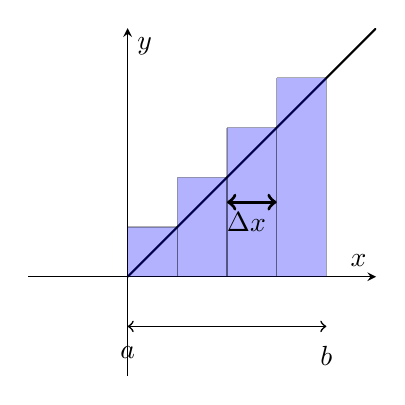
\begin{tikzpicture}
    \begin{axis}[ axis lines=center,
        xlabel = {$x$},
        ylabel = {$y$},
        xmin=-2, ymin=-2,
        xmax=5, ymax=5,
        height=6cm,
        width=6cm,
        xtick=\empty,
        ytick=\empty,
    ]
    \addplot [domain=0:5, smooth, thick] {x};
    \draw [fill=blue, opacity=0.3] (axis cs: 0,1)  -- (axis cs: 0,0) -- (axis cs: 1,0) -- (axis cs: 1,1) -- (axis cs: 0,1);
    \draw [fill=blue, opacity=0.3] (axis cs: 1,2)  -- (axis cs: 1,0) -- (axis cs: 2,0) -- (axis cs: 2,2) -- (axis cs: 1,2);
    \draw [fill=blue, opacity=0.3] (axis cs: 2,3)  -- (axis cs: 2,0) -- (axis cs: 3,0) -- (axis cs: 3,3) -- (axis cs: 2,3);
    \draw [fill=blue, opacity=0.3] (axis cs: 3,4)  -- (axis cs: 3,0) -- (axis cs: 4,0) -- (axis cs: 4,4) -- (axis cs: 3,4);
    \draw[very thick,<->] (axis cs: 2,1.5) -- (axis cs: 3,1.5) node [below left] {$\Delta x$};
    \draw [semithick,<->] (axis cs: 0,-1) -- (axis cs: 4,-1);
    \draw [semithick] (axis cs: 0,-1.2) node[below] {$a$};
    \draw [semithick] (axis cs: 4,-1.2) node[below] {$b$};
    \end{axis}
    \end{tikzpicture}
%-------Midpoint--------
    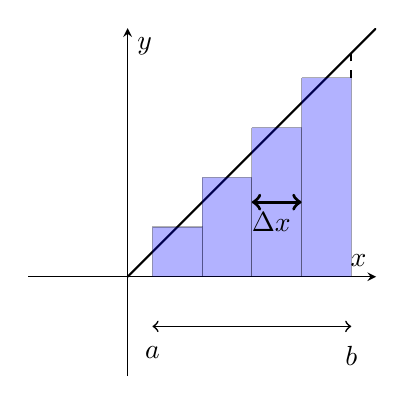
\begin{tikzpicture}
    \begin{axis}[ axis lines=center,
        xlabel = {$x$},
        ylabel = {$y$},
        xmin=-2, ymin=-2,
        xmax=5, ymax=5,
        height=6cm,
        width=6cm,
        xtick=\empty,
        ytick=\empty,
    ]
    \addplot [domain=0:5, smooth, thick] {x} node [above left] {$y=x$};
    \draw [fill=blue, opacity=0.3] (axis cs: .5,1)  -- (axis cs: .5,0) -- (axis cs: 1.5,0) -- (axis cs: 1.5,1) -- (axis cs: .5,1);
    \draw [fill=blue, opacity=0.3] (axis cs: 1.5,2)  -- (axis cs: 1.5,0) -- (axis cs: 2.5,0) -- (axis cs: 2.5,2) -- (axis cs: 1.5,2);
    \draw [fill=blue, opacity=0.3] (axis cs: 2.5,3)  -- (axis cs: 2.5,0) -- (axis cs: 3.5,0) -- (axis cs: 3.5,3) -- (axis cs: 2.5,3);
    \draw [fill=blue, opacity=0.3] (axis cs: 3.5,4)  -- (axis cs: 3.5,0) -- (axis cs: 4.5,0) -- (axis cs: 4.5,4) -- (axis cs: 3.5,4);
    \draw [dashed, semithick] (axis cs: 4.5,4) -- (axis cs: 4.5,4.5);
    \draw[very thick,<->] (axis cs: 2.5,1.5) -- (axis cs: 3.5,1.5) node [below left] {$\Delta x$};
    \draw [semithick,<->] (axis cs: .5,-1) -- (axis cs: 4.5,-1);
    \draw [semithick] (axis cs: .5,-1.2) node[below] {$a$};
    \draw [semithick] (axis cs: 4.5,-1.2) node[below] {$b$};
    \end{axis}
    \end{tikzpicture}
%-------Right endpoint--------
    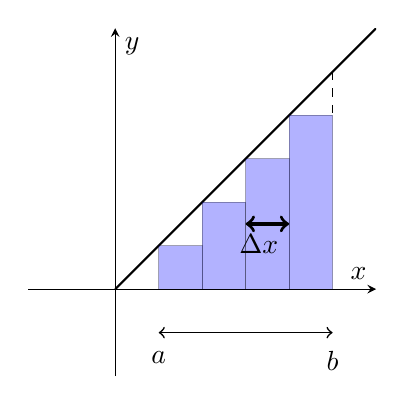
\begin{tikzpicture}
    \begin{axis}[ axis lines=center,
        xlabel = {$x$},
        ylabel = {$y$},
        xmin=-2, ymin=-2,
        xmax=6, ymax=6,
        height=6cm,
        width=6cm,
        xtick=\empty,
        ytick=\empty,
    ]
    \addplot [domain=0:6, smooth, thick] {x};
    \draw [fill=blue, opacity=0.3] (axis cs: 1,1)  -- (axis cs: 1,0) -- (axis cs: 2,0) -- (axis cs: 2,1) -- (axis cs: 1,1);
    \draw [fill=blue, opacity=0.3] (axis cs: 2,2)  -- (axis cs: 2,0) -- (axis cs: 3,0) -- (axis cs: 3,2) -- (axis cs: 2,2);
    \draw [fill=blue, opacity=0.3] (axis cs: 3,3)  -- (axis cs: 3,0) -- (axis cs: 4,0) -- (axis cs: 4,3) -- (axis cs: 3,3);
    \draw [fill=blue, opacity=0.3] (axis cs: 4,4)  -- (axis cs: 4,0) -- (axis cs: 5,0) -- (axis cs: 5,4) -- (axis cs: 4,4);
    \draw [dashed, semithick] (axis cs: 5,5) -- (axis cs: 5,4);
    \draw[very thick,<->] (axis cs: 3,1.5) -- (axis cs: 4,1.5) node [below left] {$\Delta x$};
    \draw [semithick,<->] (axis cs: 1,-1) -- (axis cs: 5,-1);
    \draw [semithick] (axis cs: 1,-1.2) node[below] {$a$};
    \draw [semithick] (axis cs: 5,-1.2) node[below] {$b$};
    \end{axis}
    \end{tikzpicture}
\end{center}


\noindent As in the figure above, the interval $\left[a, b\right]$ is divided into $n$ sub-intervals equally, so each sub-interval ($\Delta x$) has a length: $$\Delta x = \frac{b-a}{n}$$

\noindent The right endpoint location $x$ of each sub-interval will be:
\begin{align*}
    & x_1, x_2,\dots, x_{n-2}, x_{n-1}, x_n\\
    =& \left[a+\Delta x \right], \left[a+2\Delta x \right],\dots, \left[a+\left(n-2\right)\Delta x \right], \left[a+\left(n-1\right)\Delta x \right], b
\end{align*}

\noindent The right endpoint Riemann Sum:
\begin{align*}
    R_n
    &= \Delta x\left[f\left(a+\Delta x\right)+ f\left(a+2\Delta x\right)
    +\dots+ f\left(a+\left(n-1\right)\Delta x\right)+b \right]\\
    &= \Delta x\left[f\left(x_1\right)+ f\left(x_2\right)+ f\left(x_3\right)+\dots f\left(x_{n-1}\right)+ f\left(x_n\right) \right] \\
    &=\Delta x\cdot\sum_{i=1}^{n}f\left(x_i\right)\\
    &=\frac{b-a}{n}\cdot\sum_{i=1}^{n}\left(a +\frac{b-a}{n}\cdot i \right)\\
    &=\frac{b-a}{n}\cdot\left(a\sum_{i=1}^{n}1+\frac{b-a}{n}\sum_{i=1}^{n}i\right)\\
    &=\frac{b-a}{n}\cdot\left[a \cdot n+ \frac{b-a}{n}\cdot \frac{n\left(n+1\right)}{2} \right]\\
    &=\frac{b-a}{n}\cdot a\cdot n+ \frac{\left(b-a\right)^2}{n^2}\cdot \frac{n\left(n+1\right)}{2} \\
    &=a\left(b-a \right)+ \frac{n\left(b-a\right)^2+\left(b-a\right)^2}{2n} \qquad (*)\\
\end{align*}

\noindent In the equation (*), I have $n$ as the number of the sub-intervals. The more sub-intervals means that the more precise the result is, so assuming that I will divide the interval $ab$ into infinity sub-intervals. Therefore, I need to find the limit of the equation (*) when $n$ approaches infinity:
\begin{align*}
    \lim_{n\to\infty}R_n &=\lim_{n\to\infty}\left[a\left(b-a \right)+ \frac{n\left(b-a\right)^2+\left(b-a\right)^2}{2n}\right]\\
    &=\lim_{n\to\infty} \Bigg[ a\left(b-a \right)+ \frac{n \left[ \left( b-a\right)^2+ \frac{1}{n} \left(b-a\right)^2 \right]}{2n} \Bigg]\\
    &=\lim_{n\to\infty} a\left(b-a \right)+ \lim_{n\to\infty}\left[ \frac{ \left( b-a\right)^2+ \frac{1}{n} \left(b-a\right)^2}{2}\right] \\
    &=a\left(b-a \right)+ \frac{ \left( b-a\right)^2}{2} \\
    &=\frac{2a\left(b-a \right)}{2}+ \frac{ \left( b-a\right)^2}{2} \\
    &=\frac{\left(2ab-2a^2 \right)+ \left(b^2-2ab+a^2 \right)}{2} \\
    &=\frac{1}{2} \left(b^2-a^2 \right) \\
\end{align*} \par

Thus, the equation $\displaystyle \int_{a}^b x \; \mathrm{d}x= \frac{1}{2} \left(b^2-a^2 \right)$ is correct.
    
\vspace{1cm}

\subsection*{Use Riemann sums to prove that:}
$$\int_{a}^b x^2 \; \mathrm{d}x = \frac{1}{3}(b^{3}-a^{3}).$$ \par

\begin{center}
    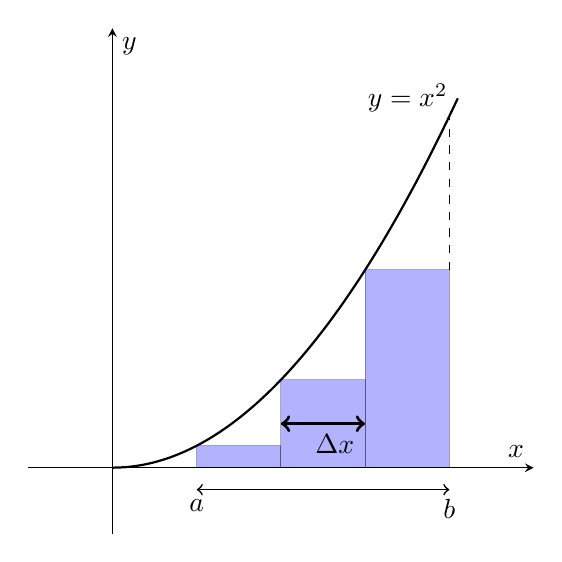
\begin{tikzpicture}
    \begin{axis}[ axis lines=center,
        xlabel = {$x$},
        ylabel = {$y$},
        xmin=-1, ymin=-3,
        xmax=5, ymax=20,
        height=8cm,
        width=8cm,
        xtick=\empty,
        ytick=\empty,
    ]
    \addplot [domain=0:4.1, smooth, thick] {x^2} node [left] {$y=x^2$};
    \draw [fill=blue, opacity=0.3] (axis cs: 1,1)  -- (axis cs: 1,0) -- (axis cs: 2,0) -- (axis cs: 2,1) -- (axis cs: 1,1);
    \draw [fill=blue, opacity=0.3] (axis cs: 2,4)  -- (axis cs: 2,0) -- (axis cs: 3,0) -- (axis cs: 3,4) -- (axis cs: 2,4);
    \draw [fill=blue, opacity=0.3] (axis cs: 3,9)  -- (axis cs: 3,0) -- (axis cs: 4,0) -- (axis cs: 4,9) -- (axis cs: 3,9);
    \draw [dashed, semithick] (axis cs: 4,9) -- (axis cs: 4,16);
    \draw[very thick,<->] (axis cs: 2,2) -- (axis cs: 3,2) node [below left] {$\Delta x$};
    \draw [semithick,<->] (axis cs: 1,-1) -- (axis cs: 4,-1);
    \draw [semithick] (axis cs: 1,-1) node[below] {$a$};
    \draw [semithick] (axis cs: 4,-1) node[below] {$b$};
    \end{axis}
    \end{tikzpicture}
\end{center}

Similarly to question 1: \par
\begin{align*}
    R_n &=\Delta x\cdot\sum_{i=1}^{n}f\left(x_i\right)^2\\
    &=\frac{b-a}{n}\cdot\sum_{i=1}^{n}\left(a +\frac{b-a}{n}\cdot i \right)^2\\
    &=\frac{b-a}{n}\cdot\sum_{i=1}^{n}\left(a^2+ 2a\cdot \frac{b-a}{n} \cdot i +\frac{\left( b-a\right)^2}{n^2}\cdot i^2 \right)\\
    &=\frac{b-a}{n}\left(a^2\cdot \sum_{i=1}^{n}1+ 2a\cdot \frac{b-a}{n}\cdot \sum_{i=1}^{n}i +\frac{\left( b-a\right)^2}{n^2}\cdot \sum_{i=1}^{n}i^2 \right)\\
    &=\frac{b-a}{n}\left(a^2\cdot n+ 2a\cdot \frac{b-a}{n}\cdot \frac{n\left( n+1\right)}{2} +\frac{\left( b-a\right)^2}{n^2}\cdot \frac{n\left( n+1\right) \left( 2n+1\right)}{6} \right)\\
    &=a^2\left( b-a\right)
    + \frac{n\cdot2a\left( b-a\right)^2+2a\left(b-a \right)^2}{2n}
    + \frac{2n^2\left(b-a\right)^3+ 3n\left(b-a\right)^3+ \left(b-a\right)^3}{6n^2}\\
    &=a^2\left( b-a\right)
    + a\left(b-a\right)^2\left(1+ \frac{1}{n}\right)
    + \frac{\left(b-a\right)^3 \left(2+\frac{3}{n}+ \frac{1}{n^3} \right)}{6}
\end{align*}


\begin{align*}
    \lim_{n\to\infty}R_n 
    &=\lim_{n\to\infty} a^2\left( b-a\right)
    + \lim_{n\to\infty}\left[ a\left(b-a\right)^2 \left(1+ \frac{1}{n} \right)\right]
    + \lim_{n\to\infty}\left[ \frac{\left(b-a\right)^3 \left(2+\frac{3}{n}+ \frac{1}{n^3} \right)}{6} \right]\\
    &=\left(a^2b-a^3\right)
    + \left(ab^2-2a^2b+a^3\right)
    + \frac{1}{3}\left(b^3-3ab^2+3a^2b-a^3\right)\\
    &= \frac{1}{3} \left(3a^2b-3a^3+ 3ab^2-6a^2b+3a^3+ b^3-3ab^2+3a^2b-a^3 \right)\\
    &= \frac{1}{3}\left(b^3-a^3\right)
\end{align*} 

Thus, the equation $\displaystyle \int_{a}^b x^2 \; \mathrm{d}x= \frac{1}{3} \left(b^3-a^3 \right)$ is correct.\paragraph{}

\vspace{1cm}

\subsection*{Use Riemann sums to prove that:}
$$\int_{a}^b x^3 \; \mathrm{d}x = \frac{1}{4}(b^{4}-a^{4}).$$ \par

\begin{center}
    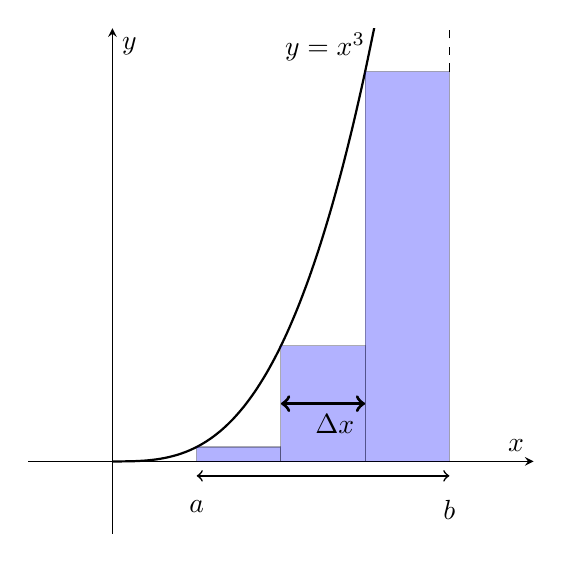
\begin{tikzpicture}
    \begin{axis}[ axis lines=center,
        xlabel = {$x$},
        ylabel = {$y$},
        xmin=-1, ymin=-5,
        xmax=5, ymax=30,
        height=8cm,
        width=8cm,
        xtick=\empty,
        ytick=\empty,
    ]
    \addplot [domain=0:3.12, smooth, thick] {x^3} node [below left] {$y=x^3$};
    \draw [fill=blue, opacity=0.3] (axis cs: 1,1)  -- (axis cs: 1,0) -- (axis cs: 2,0) -- (axis cs: 2,1) -- (axis cs: 1,1);
    \draw [fill=blue, opacity=0.3] (axis cs: 2,8)  -- (axis cs: 2,0) -- (axis cs: 3,0) -- (axis cs: 3,8) -- (axis cs: 2,8);
    \draw [fill=blue, opacity=0.3] (axis cs: 3,27)  -- (axis cs: 3,0) -- (axis cs: 4,0) -- (axis cs: 4,27) -- (axis cs: 3,27);
    \draw [dashed, semithick] (axis cs: 4,27) -- (axis cs: 4,30);
    \draw[very thick,<->] (axis cs: 2,4) -- (axis cs: 3,4) node [below left] {$\Delta x$};
    \draw [semithick,<->] (axis cs: 1,-1) -- (axis cs: 4,-1);
    \draw [semithick] (axis cs: 1,-2) node[below] {$a$};
    \draw [semithick] (axis cs: 4,-2) node[below] {$b$};
    \end{axis}
    \end{tikzpicture}
\end{center}

Similarly to question 1: \par
\begin{align*}
    \begin{split}
        R_n &=\Delta x\cdot\sum_{i=1}^{n}f\left(x_i\right)^3\\
        &=\frac{b-a}{n}\cdot\sum_{i=1}^{n}\left(a +\frac{b-a}{n}\cdot i \right)^3\\
        &=\frac{b-a}{n}\cdot\sum_{i=1}^{n} \left[a^3+ 3a^2\cdot i\cdot\frac{b-a}{n}+ 3a\cdot i^2\cdot\frac{\left(b-a\right)^2}{n^2} + i^3\cdot\frac{\left(b-a\right)^3}{n^3}\right]\\
        &=\frac{b-a}{n}\left[ a^3\sum_{i=1}^{n}1 
        + \frac{3a^2\left(b-a\right)}{n} \sum_{i=1}^{n}i
        + \frac{3a\left(b-a\right)^2}{n^2} \sum_{i=1}^{n}i^2
        + \frac{\left(b-a\right)^3}{n^3} \sum_{i=1}^{n}i^3 \right]\\
        &=\frac{a^3\left(b-a\right)}{n}\cdot n
        + \frac{3a^2\left(b-a\right)^2}{n^2} \cdot\frac{n\left(n+1\right)}{2}
        + \frac{3a\left(b-a\right)^3}{n^3} \cdot\frac{n\left(n+1\right)\left(2n+1\right)}{6}\\
        &\qquad\qquad\qquad\qquad\qquad\qquad\qquad\qquad\qquad\qquad
        \qquad\quad
        + \frac{\left(b-a\right)^4}{n^4} \cdot \frac{n^2\left(n+1 \right)^2}{4}\\
        &=a^3\left(b-a\right)
        + \frac{3}{2} a^2\left(b-a\right)^2 \left(1+\frac{1}{n}\right)
        + \frac{1}{2} a\left(b-a\right)^3 \left(2+ \frac{3}{n}+ \frac{1}{n^2} \right) \\
        &\qquad\qquad\qquad\qquad\qquad\qquad\qquad\qquad
        \qquad\qquad\qquad
        + \frac{1}{4} \left(b-a\right)^4 \left(1+ \frac{2}{n}+ \frac{1}{n^2} \right)
    \end{split}
\end{align*}

\begin{align*}
    \lim_{n\to\infty}R_n &=a^3\left(b-a\right)
    + \frac{3}{2} a^2\left(b-a\right)^2 \lim_{n\to\infty}\left(1+\frac{1}{n}\right)
    + \frac{1}{2} a\left(b-a\right)^3 \lim_{n\to\infty}\left(2+ \frac{3}{n}+ \frac{1}{n^2} \right)\\
    &\qquad\qquad\qquad\qquad\qquad\qquad\qquad\qquad
    \qquad\quad
    +\frac{1}{4} \left(b-a\right)^4 \lim_{n\to\infty} \left(1+ \frac{2}{n}+ \frac{1}{n^2} \right)\\
    &=\left(a^3b-a^4\right) 
    + \frac{3}{2} \left(a^2b^2-2a^3b+a^4\right)
    + \left(ab^3-3a^2b^2+3a^3b-a^4\right) \\
    &\qquad\qquad\qquad\qquad\qquad\qquad\qquad\qquad
    \qquad
    + \frac{1}{4} \left(b^4-4ab^3+6a^2b^2-4a^3b+a^4 \right) \\
    &= \frac{1}{4} \left(4a^3b-4a^4\right)
    + \frac{1}{4} \left(6a^2b^2-12a^3b+6a^4\right)\\
    &\qquad\quad
    + \frac{1}{4} \left(4ab^3-12a^2b^2+12a^3b-4a^4\right)
    + \frac{1}{4} \left(b^4-4ab^3+6a^2b^2-4a^3b+a^4 \right) \\
    &=\frac{1}{4} \left(b^4-a^4 \right)
\end{align*}

\noindent Thus, the equation $\displaystyle \int_{a}^b x^3 \; \mathrm{d}x= \frac{1}{4} \left(b^4-a^4 \right)$ is correct.\par

\vspace{1cm}

\subsection*{Conclusion:}

\noindent With $\displaystyle k=1: \int_{a}^b x \; \mathrm{d}x = \frac{1}{2}(b^{2}-a^{2}).
\Longleftrightarrow \int_{a}^b x^1 \; \mathrm{d}x = \frac{1}{1+1}(b^{1+1}-a^{1+1}).$ \par

\noindent With $\displaystyle k=2: \int_{a}^b x^2 \; \mathrm{d}x = \frac{1}{3}(b^{3}-a^{3}).
\Longleftrightarrow \int_{a}^b x^2 \; \mathrm{d}x = \frac{1}{2+1}(b^{2+1}-a^{2+1}).$ \par

\noindent With $\displaystyle k=3: \int_{a}^b x^3 \; \mathrm{d}x = \frac{1}{4}(b^{4}-a^{4}).
\Longleftrightarrow \int_{a}^b x^3 \; \mathrm{d}x = \frac{1}{3+1}(b^{3+1}-a^{3+1}).$ \par

\noindent It is obvious that for every integral of $x^k$ from $a$ to $b$, the result is always equal to: $$\displaystyle \frac{1}{k+1} \left(b^{k+1}-a^{k+1} \right)$$. \par

\noindent Therefore, the equation $\displaystyle \int_{a}^b x^k \; \mathrm{d}x= \frac{1}{k+1} \left(b^{k+1}-a^{k+1} \right)$ is correct.
    



%___________EXAM_3___________
\newpage

\hrule
\vspace{.2mm}
\begin{center}
    \section*{Different Viewpoints}
    \textit{Quan H. Nguyen}
\end{center}
\vspace{.2mm}
\hrule

\subsection*{Introduction to the problem:}

\noindent We need to find the volume of an object which is described to be a circular shape viewing from the top, a square from the front, and a triangle from its side. To calculate the volume, it is necessary to know its cross section, which can be either a square, or a triangle.

\subsection*{Case 1:}
    
\subsubsection*{Description:}
    
\noindent Viewing from the top, the object has circle shape with $r$ as its radius.
    
\noindent From the front, that object looks like a square whose side lengths are the same as the diameter of the circle: $2r$, so the size of that square is $2r$ x $2r$.
    
\noindent The cross section of this object is a equilateral triangle (side view on $xz$ plane) because its height $OS$ is a midperpendicular line to the base with $O$ is the center of the based circle. As the cross section moves away from the origin and along the $y$-axis, its height remains the same as the square's height ($OS=2r$), but its base becomes smaller depending on the circle.
    

    %------------------------------------------
\begin{center}
\tdplotsetmaincoords{70}{110}
\begin{tikzpicture}[tdplot_main_coords, scale =1]

    \draw[thick,->] (-5,0,0) -- (5,0,0) node[below left]{$x$};
    \draw[thick,->] (0,-5,0) -- (0,5,0) node[below left]{$y$};
    \draw[thick,->] (0,0,-2) -- (0,0,7) node[below left]{$z$};
    \draw (0,0,0) node[below left, color=gray]{$O$};
    \draw (0,3,0) node[below right]{$r$};
    \draw (0,-3,0) node[above left]{$-r$};
    \draw (0,0,6) node[above right]{S$(0,0,2r)$};
    \draw (3,0,0) node[below right]{$r$};
        
    % The base
    \draw[dashed,color=gray] (0,-3,0) arc (270:90:3 and 3);
    \draw[semithick] (0,-3,0) arc (-90:90:3 and 3);
	    
    % The square
    \draw[semithick] (0,-3,0) -- (0,-3,6);
    \draw[semithick] (0,3,0) -- (0,3,6);
    \draw[semithick] (0,-3,6) -- (0,3,6);
	    
    % Triangles
    \filldraw[draw=black, fill=gray, opacity=0.2] (3,0,0) -- (-3,0,0) -- (0,0,6);
    \filldraw[draw=black, fill=gray, opacity=0.6] (2.5981,1.5,0) -- (-2.5981,1.5,0) -- (0,1.5,6);
    \draw[semithick] (0,1.5,0) -- (0,1.5,6);
    \draw[draw=gray, thick] (2.5981,1.5,0) -- (0,1.5,0);
    \draw[dashed, draw=gray, thin] (2.5981,1.5,0) -- (2.5981,0,0);
    \draw (0,1.5,0) node[above right]{B($0,y,0$)};
    \draw (2.5981,1.5,0) node[below right]{A($x,y,0$)};
    \draw (-2.5981,1.5,0) node[above right]{C($-x,y,0$)};

\end{tikzpicture}
\end{center}

    %------------------------
    
\subsubsection*{Volume:}
\begin{itemize}
    \item The length of cross section's base: \par
    Here is the equation of the circle on $xy$ plane:
    \begin{align*}
        x^2+y^2&=r^2 \\
        \Longleftrightarrow
        x^2&=r^2-y^2 \\
        \Longleftrightarrow
        x&=\pm \sqrt{r^2-y^2}\\
    \end{align*}
    $\Longrightarrow$ $x$ is also the equation to find the length of $AB$. The length of AB must be positive, so the length of AB has the equation: $|x|=\sqrt{r^2-y^2}$.\par
    
    However, the cross section's base (triangle's base) is equal to the length of $AC$. Since the triangle is equilateral, $AC$ is equal to $2AB$. Thus, the length of the triangle's base $AC$ is: $$2|x|=2\sqrt{r^2-y^2}$$
    
    \item Area of the cross section (triangle):
    \begin{align*}
        \text{A}(y) &=\frac{1}{2}\left(\text{height}\cdot\text{base} \right)\\
        &=\frac{1}{2}\left(OS\cdot AC\right)\\
        &=\frac{1}{2}\left(2r\cdot 2\sqrt{r^2-y^2} \right)\\
        &= 2r\sqrt{r^2-y^2}\\
    \end{align*}
    
    \item Volume of the object: \par
    Since the object is symmetric about $z$-axis on $yz$ plane, the object's volume from $-r \to 0$ is equal to object's volume from $0\to r$ on $y$-axis. \par
    \begin{align*}
        \mathrm{V}(y) = \int_{-r}^r \mathrm{A}(y)\; \mathrm{d}y
        &=2 \int_{0}^r \mathrm{A}(y)\; \mathrm{d}y \\
        &=2 \int_{0}^r 2r\sqrt{r^2-y^2} \; \mathrm{d}y\\
        &=4r \int_{0}^r \sqrt{r^2-y^2} \; \mathrm{d}y
    \end{align*}
    
    I let $y=r\sin{t}$ because when squaring both sides of the equation, $``y"\to ``y^2"$ and $``r\sin{t}"\to ``r^2\sin^2{t}"$. Then leave $r^2$ as factor, $1-\sin^2{t}=\cos^2{t}$ which cancels the square root: \par
    
    \begin{equation*}
        y=r\sin{t}\\
        \Longleftrightarrow
        \begin{cases}
            \mathrm{d}y = r \cos{t}\; \mathrm{d}t\\
            t=\arcsin{\frac{y}{r}}
        \end{cases}
    \end{equation*}
    
    
    \begin{align*}
        \mathrm{V}(y) &= 4r \int_{0}^r \sqrt{r^2-y^2} \; \mathrm{d}y \\
        \Longrightarrow \mathrm{V}(y)&= 4r \int_{0}^r r\cos{t}\cdot\sqrt{r^2-r^2\sin^2{t}} \; \mathrm{d}t \\
        &= 4r \int_{0}^r r\cos{t}\cdot \sqrt{r^2 \left(1-\sin^2{t}\right)} \; \mathrm{d}t \\
        &= 4r \int_{0}^r r\cos{t}\cdot\sqrt{r^2 \cos^2{t}} \; \mathrm{d}t \\
        &= 4r \int_{0}^r r\cos{t}\cdot r \cos{t} \; \mathrm{d}t \\
        &= 4r \int_{0}^r r^2 \cos^2{t}\; \mathrm{d}t \\
        &= 4r^3 \int_{0}^r \cos^2{t}\; \mathrm{d}t \\
        &= 4r^3 \int_{0}^r \frac{1+\cos{2t}}{2}\; \mathrm{d}t \\
        &= 2r^3\int_{0}^r 1\; \mathrm{d}t +2r^3 \int_{0}^r \cos{2t}\; \mathrm{d}t \\
        &= 2r^3\int_{0}^r 1\; \mathrm{d}t
        +r^3 \int_{0}^r 2\cos{2t}\; \mathrm{d}t \\
        &= \left(2r^3 t \right)_0^r
        +\left(r^3 \sin{2t} \right)_0^r \\
        &= \left(2r^3 \arcsin{\frac{y}{r}}
        \right)_0^r
        +\left[r^3 \sin{\left( 2\arcsin{\frac{y}{r}} \right)} \right]_0^r \\
        &= \left(2r^3\cdot \frac{\pi}{2}-0 \right)
        +\left(0-0 \right) \\
        &= \pi r^3 \\
    \end{align*}
    
\end{itemize}
    
\noindent In summary, the volume of the object that has triangle cross sections is $\pi r^3$.

%------------CASE 2---------------

\vspace{1cm}

\subsection*{Case 2:}
    
\subsubsection*{Description:}

\noindent Viewing from the top, the object has circle shape with $r$ as its radius, which is the same as Case 1.
        
\noindent However, from the front in Case 2, the object now is a equilateral triangle. The triangle has base length of $2r$ (equal to diameter of the based circle) and height of $2r$ so that it can create a $2r$ x $2r$ square when viewing from the side. The triangle is equilateral because its height is also $Oz$-axis, which is midperpendicular to the base.
        
\noindent The cross section of this object is a square (side view) with the size of $2r$ x $2r$ on the $xz$ plane as I explained above. That cross section when moving away from origin $O$, along the $y$-axis, it loses square shape because its height decrease steadily due to triangle's side while its base decrease exponentially due to the circle.
    
%--------------------------
\begin{center}
\tdplotsetmaincoords{70}{110}
\begin{tikzpicture}[tdplot_main_coords, scale =1]
    \draw[thick,->] (-5,0,0) -- (5,0,0) node[below left]{$x$};
    \draw[thick,->] (0,-5,0) -- (0,5,0) node[below left]{$y$};
    \draw[thick,->] (0,0,-2) -- (0,0,7) node[below left]{$z$};
        
    % The base
    \draw[dashed,color=gray] (0,-3,0) arc (270:90:3 and 3);
    \draw[semithick] (0,-3,0) arc (-90:90:3 and 3);
    \draw (0,0,0) node[below left]{$O$};
    \draw (0,3,0) node[above right]{B($0,r,0$)};
    \draw (0,-3,0) node[above left]{$-r$};
    \draw (0,0,6) node[left]{A($0,0,2r$)};
	
    % The triangle
    \draw[semithick] (0,-3,0) -- (0,0,6);
    \draw[semithick] (0,3,0) -- (0,0,6);

    % Squares
    \filldraw[draw=black, fill=gray, opacity=0.2] (3,0,0) -- (-3,0,0) -- (-3,0,6) -- (3,0,6);
    \filldraw[draw=black, fill=gray, opacity=0.6] (2.5981,1.5,0) -- (-2.5981,1.5,0) -- (-2.5981,1.5,3) -- (2.5981,1.5,3);
    \draw[semithick] (-2.5981,1.5,0) -- (2.5981,1.5,0);
    \draw[semithick] (0,1.5,0) -- (0,1.5,3);

\end{tikzpicture}
\end{center}

%----------------------------
    
    
\subsubsection*{Volume:}
\begin{itemize}
    \item Height of the cross section:\par
    
    Because the triangle (on $yz$ plane) is symmetric about $z$-axis, the change in cross section's height from $O\to -r$ is the same as that from $O\to r$, so I only need to find the equation of the line $AB$ (from $O\to r$).
    
    The general formula of linear line $AB$: $$z = my + b$$ \par
    
    The $z$ intercept of the line $AB$ on $yz$ plane is $A(0,0,2r)$, and the $y$ intercept is $B(0,r,0)$. Plug these two coordinations into the general formula, I have a system of two equations:
    \begin{equation*}
        \begin{cases}
            2r=0 + b\\
            0=rm+b
        \end{cases} \\
        \Longleftrightarrow
        \begin{cases}
            b=2r\\
            m=-2
        \end{cases}
    \end{equation*}

Therefore, the equation for height of square is:
$$z=-2y+2r$$
    

    \item Equation for base of the cross section (on $xy$ plane), same as in Case 1:
    $$2x=2\sqrt{r^2-y^2}$$ \par
    
    \item Area of cross section (rectangle): 
    \begin{align*}
        \mathrm{A}(y)&=\text{height} \cdot \text{base}\\
        &=z\cdot 2x \\
        &=\left(-2y+2r\right)\cdot 2\sqrt{r^2-y^2}\\
        &= 4\left(r-y\right)\sqrt{r^2-y^2}\\
        &= 4r\sqrt{r^2-y^2}-4y\sqrt{r^2-y^2}
    \end{align*}
    
    \item Volume of the object (similar to Case 1):. \par
    \begin{align*}
        \mathrm{V}(y) = \int_{-r}^r \mathrm{A}(y)\; \mathrm{d}y
        &=2 \int_{0}^r \mathrm{A}(y)\; \mathrm{d}y \\
        &=2 \int_{0}^r\left( 4r\sqrt{r^2-y^2}-4y\sqrt{r^2-y^2}\right) \; \mathrm{d}y\\
        &=2\cdot 4r \int_{0}^r \sqrt{r^2-y^2}\; \mathrm{d}y
        - 8\int_{0}^r y\sqrt{r^2-y^2} \; \mathrm{d}y\\
        &=2\pi r^3
        - 8\int_{0}^r y\sqrt{r^2-y^2} \; \mathrm{d}y
        \quad \left(4r \int_{0}^r \sqrt{r^2-y^2} \; \mathrm{d}y=\pi r^3\right)
    \end{align*}
    
    Assuming that:
    \begin{align*}
        &t=\sqrt{r^2-y^2}\\
        \Longrightarrow &t^2 = r^2-y^2\\
        \Longrightarrow &2t\; \mathrm{d}t = -2y\;\mathrm{d}y\\
        \Longrightarrow &t\; \mathrm{d}t = -y\;\mathrm{d}y\\
    \end{align*}
    
    \begin{align*}
        \mathrm{V}(y) &=2\pi r^3
        - 8\int_{0}^r y\sqrt{r^2-y^2} \; \mathrm{d}y\\
        \Longrightarrow \mathrm{V}(y)
        &=2\pi r^3
        + 8\int_{0}^r t^2 \; \mathrm{d}t\\
        &=2\pi r^3
        + 8\left(\frac{t^3}{3}\right)_0^r\\
        &=2\pi r^3
        + \frac{8}{3}\left[\left(r^2-y^2 \right) \sqrt{r^2-y^2}\right]_0^r \\
        &=2\pi r^3
        + \frac{8}{3}\left(0 -r^2 \sqrt{r^2} \right) \\
        &=2\pi r^3- \frac{8}{3}r^3\\
        &=2r^3 \left(\pi -\frac{4}{3}\right)
    \end{align*}

\end{itemize}
    
\noindent In summary, the volume of the object that has rectangle cross sections is $ 2r^3\left(\pi -\frac{4}{3}\right)$.
    

    
%___________EXAM_4_______________
\newpage

\hrule
\vspace{.2mm}
\begin{center}
    \section*{Probability -- Prove Your Ability}
    \textit{Quan H. Nguyen}
\end{center}
\vspace{.2mm}
\hrule


Some formulas and conventions that I use in this exam:
\begin{itemize}
    \item The mean score (average score):
    $$=\frac{\text{Total scores}}{\text{Total number of student}}$$
    \item The probability: 
    $$=\frac{\text{Number of student scored a 7 or higher}}{\text{Total number of student took exam}}$$
    \item All numbers are rounded to the nearest one.
    \item The total number of student taking the exam is equal to the total frequency of all scores from 0 to 10.
    \item All numbers with decimal are rounded to the nearest one.
\end{itemize}


\subsection*{Combinatorics class}
\begin{center}
    \begin{tabular}{l | c*{10}r}
        Score &0 &1 &2 &3 &4 &5 &6 &7 &8 &9 &10 \\
        \hline
        Frequency &0 &1 &0 &1 &1 &2 &3 &5 &4 &2 &1
    \end{tabular}
\end{center}


\begin{enumerate}
    \item Number of students scored a 7: $5$.
    
    \item Number of students scored a 7 or higher: $12$.\par
    Explain: 5 students scored a 7; 4 students scored a 8; 2 students scored a 9; 1 students scored a 10.
        
    \item Number of students took the exam: 20. \par
    Explain: The number of students took the exam is equal to the total frequency of all scores from $1 \to 10$
        
    \item The most frequent score: $7$ \par
    Explain: The highest frequency is 5. The score with 5 in frequency is 7.
        
    \item Probability = $\frac{12}{20}= \frac{3}{5}$.
        
    \item The mean score = $\frac{1\cdot 1+3\cdot 1+4\cdot 1+5\cdot 2+6\cdot 3+7\cdot 5+8\cdot 4+9\cdot 2+10\cdot 1}{20}=
    \frac{131}{20} = 6.55$.
        
    \item There are 20 numbers in total, so the middle number will be a number that is in the middle of 10th and 11th number counting from score of $0\to 10$ \par
    The middle = $\frac{7+7}{2} = 7$
        
    \begin{center}
        \begin{tabular}{l | c|c|c|c|c|c|c|c|c|c |r}
            Score & 1 & 3 & 4 & 5 & \dots & 6 & 7 & 7 & 7 & \dots & 10 \\
            \hline
            &1st &2nd &3rd &4th &\dots &8th &9th &10th &11th &\dots &20th \\
        \end{tabular}
    \end{center}
        
    \vspace{0.5cm}

\end{enumerate}

\vspace{1cm}
    
\subsection*{Probability class}
The general equation to calculate number of students (frequency) who scored n points: $$f(n)=\frac{15n-n^2}{2}$$ \par
\begin{center}
    \begin{tabular}{l | c*{10}r}
        Score ($n$) & 0 & 1 & 2 & 3 & 4 & 5 & 6 & 7 & 8 & 9 & 10 \\
        \hline
        Frequency ($f(n)$)
        &0 &7 &13 &18 &22 &25 &27 &28 &28 &27 &25 \\
    \end{tabular}
\end{center}


\begin{enumerate}
    \item Number of students scored a 7: 28.
        
    \item Number of students scored a 7 or higher: 108.\par
    $$\sum_{x=7}^{10}\frac{15x-x^2}{2}=108$$
        
    \item 
    Number of students took the exam: 220.\par
    $$\sum_{x=0}^{10}\frac{15x-x^2}{2}=220$$
            
        
    \item The most frequent score is 7 and 8. \par
    Explain: 28 students scored 7 and 28 students scored 8. 28 was also the most frequent score.
        

    \item Probability: $$=\;\frac{108}{220}\;=\;\frac{27}{55}$$
        
    \item The mean:
    $$=\frac{0+(1\cdot 7)+(2\cdot 13)+(3\cdot 18)+\cdots+(8\cdot 28)+(9\cdot 27)+(10\cdot 25)}{220}
    =\frac{25}{4}
    =6.25$$
        
    \item There are 220 students taking the exam, so the middle number will be a number that is in the middle of 110th and 111th number counting from score of $0 \to 10$\par
    The middle: $$=\frac{6+6}{2}=6$$
        
    \begin{center}
        \begin{tabular}{l |c|c|c|c|c|c|c|c|c|c|c| r}
            Score & 1 & 1 & 1 & 1 & \dots & 6 & 6 & 6 & 7 & \dots & 10 \\
            \hline
            &1st &2nd &3rd &4th &\dots &110th &111th &112th &113th &\dots &220th \\
        \end{tabular}
    \end{center}
        
\end{enumerate}

\vspace{1cm}

\subsection*{Statistic class}
The general equation to calculate number of students (frequency) who scored $x$ points: $$f(x)=63e^{\frac{ -\left(x-7 \right)^2}{4}} $$ \par
\begin{center}
    \begin{tabular}{l | c*{10}r}
        Score ($x$) & 0 & 1 & 2 & 3 & 4 & 5 & 6 & 7 & 8 & 9 & 10 \\
        \hline
        Frequency &0 &0 &0 &1 &7 &24 &49 &62 &49 &24 &7 \\
    \end{tabular}
\end{center}

\begin{enumerate}
    \item Number of students scored a 7: $$\int_{6.5}^{7.5} f(x)\;\mathrm{d}x = 61.7=62
    \qquad (\text{rounded to the nearest 1})$$. \par

    \item Number of students scored a 7 or higher (equal to sum number of students scored 7, 8, 9, and 10): 
    \begin{align*}
        &\int_{6.5}^{7.5} f(x)\;\mathrm{d}x 
        + \int_{7.5}^{8.5} f(x)\;\mathrm{d}x
        + \int_{8.5}^{9.5} f(x)\;\mathrm{d}x
        + \int_{9.5}^{10} f(x)\;\mathrm{d}x \\
        =\quad& \int_{6.5}^{10} f(x)\;\mathrm{d}x \\
        =\quad& 138.7 \\
        =\quad& 139 \qquad (\text{rounded to the nearest 1})
    \end{align*}

    \item Number of students took the exam (equal to total number of students scored from $0\to 10$):
    \begin{align*}
        &\int_{0}^{0.5} f(x)\;\mathrm{d}x 
        + \int_{0.5}^{1.5} f(x)\;\mathrm{d}x 
        +\cdots
        + \int_{8.5}^{9.5} f(x)\;\mathrm{d}x
        + \int_{9.5}^{10} f(x)\;\mathrm{d}x \\
        =\quad&\int_{0}^{10} f(x)\;\mathrm{d}x \\
        =\quad& 219.5 \\
        =\quad& 220 \qquad (\text{rounded to the nearest 1})
    \end{align*}
        
        
    \item The most frequent score: 7. Because the highest frequency was 62 and 62 students scored 7.
        
    \item Probability:
    $$\left(\int_{6.5}^{10} f(x)\;\mathrm{d}x \right) 
    \;\div 
    \left(\int_{0}^{10} f(x)\;\mathrm{d}x \right)
    = \frac{139}{220}$$

        
    \item The mean:
    \begin{align*}
        &=\left( \int_0^{10}x\cdot f(x) \;\mathrm{d} x\right)
        \div
        \left(\int_0^{10} f(x) \;\mathrm{d}x \right) \\
        &= \frac{1}{220} \int_0^{10}x\cdot f(x) \;\mathrm{d}x \\
        &= 6.93
    \end{align*}
        

    \item There are 220 students taking the exam, so the middle number will be a number that is in the middle of 110th and 111th number counting from score of $0 \to 10$. \par
    The middle $$=\frac{7+7}{2}= 7 $$
        
    \begin{center}
        \begin{tabular}{l | c|c|c|c|c|c|c|c|c|c |r}
            Score & 3 & 4 & 4 & 4 & 4 & \dots & 7 & 7 & \dots & 10 \\
            \hline
            &1st &2nd &3rd &4th &5th &\dots &110th &111th &\dots & 220th \\
        \end{tabular}
    \end{center}
        
\end{enumerate}



%_____________EXAM_5______________
\newpage

\hrule
\vspace{.2mm}
\begin{center}
    \section*{Solitaire Army}
    \textit{Quan H. Nguyen}
\end{center}
\vspace{.2mm}
\hrule

\subsection*{Introduction to the problem:}

\noindent This problem is from a game named Solitaire Army  playing on a infinite board, which was created by John Conway in 1961. In this game, we move the pegs by jumping over another peg (only horizontally or vertically). The peg that is jumped over is removed, so this results in reducing 1 peg after each move. It is only possible to move the pegs to the point from the 1st to the 4th row on the other side of the demarcation line. I will prove why that happens in the section below.

\noindent Assuming that:
\begin{itemize}
    \item The cell I want to move the peg to is $1$.
    \item $i$ (a positive number) is the value of the cell containing it.
    \item For every cell that is further than 1, the value of that cell is multiplied by $i$.
\end{itemize}

\vspace{1cm}

\subsection*{Moving the peg to the 1st row:}
\begin{center}
\begin{tabular}{|l|c|c|c|c|c|c|c|c|c|c|r|}
    \hline
    $i^2$ \\
    \hline
    $i$ \\
    \hline
    $1$ \\
    \hline
\end{tabular}
\end{center}

\begin{itemize}
    \item From the table above, I have $i+i^2=1$
    
    The value of $i$ (using the equation above): \par
    
    \begin{align*}
        i+i^2&=1\\
        \Longleftrightarrow
        i^2+i-1&=0\\
    \end{align*}

    \noindent $i^2+i-1=0$ has the general quadratic equation: $ax^2+bx+c=0$, which means that $a=1$, $b=1$, and $c=-1$. The quadratic formula that is used to find the value of $i$:

    \begin{align*}
        & i = \frac{-b\pm \sqrt{b^2-4ac}}{2a} \\
        \Longleftrightarrow\;
        & i = \frac{-1\pm \sqrt{\left(-1\right)^2 -4\cdot 1 \cdot (-1)}}{2\cdot 1}\\
        \Longleftrightarrow\;
        & i_1 = \frac{-1\pm\sqrt{5}}{2}\\
        \Longleftrightarrow\;
        & i_1 = -1.618034
        \quad \lor\quad i_2 = 0.618034
    \end{align*}


    \noindent From what I assumed at the beginning:
    \begin{align*}
        &
        \begin{cases}
            1=i^2+i \\
            i>0
        \end{cases}\\
        \Longrightarrow &
        \begin{cases}
            1>i\\
            1>0
        \end{cases}\\
        \Longrightarrow & 1>i>0\\
        \Longrightarrow & i= i_2=0.618033
    \end{align*}

    \noindent Because $0<i<1$, $i^2$ must be smaller than $i$:
    $$0<i^2<i<1$$

    \noindent Similarly, $i^n$ with $n\to \infty$ will result in:
    $$0<i^n<i^{n-1}<\dots<i^3<i^2<i<1$$
\end{itemize}

\vspace{1cm}

\subsection*{Moving the peg to the 2nd row:}

\noindent I can move the pegs to the 2nd row with 4 pegs: 1 peg $i^2$, 2 pegs $i^3$, and 1 peg $i^4$:

\begin{center}
\begin{tabular}{|l|c|c|c|c|c|c|c|c|c|c|r|}
    \hline
    $i^3$ &  & \\
    \hline
    $i^2$ & $i^3$ & $i^4$  \\
    \hline
    &  &  \\
    \hline
    $1$ &  &  \\
    \hline
\end{tabular}
$\longrightarrow$
\begin{tabular}{|l|c|c|c|c|c|c|c|c|c|c|r|}
    \hline
    &  & \\
    \hline
    & $i^3$ & $i^4$  \\
    \hline
    \color{red}{$i$} &  &  \\
    \hline
    $1$ &  &  \\
    \hline
\end{tabular}
$\longrightarrow$
\begin{tabular}{|l|c|c|c|c|c|c|c|c|c|c|r|}
    \hline
    \\
    \hline
    \color{red}{$i^2$} \\
    \hline
    $i$ \\
    \hline
    $1$ \\
    \hline
\end{tabular}

\noindent *Note: Red pegs are new moves.
\end{center}


\noindent Checking:
\begin{align*}
    i^2+2i^3+i^4 &= i^2+i^3+i^3+i^4\\
    &= i \left(i+i^2 \right)+i^2 \left(i+i^2 \right)\\
    &=i+ i^2\\
    &= 1
\end{align*}


\noindent *As I can convert $i^2+i^3=i$ and $i^3+i^4=i^2$, I can now use the formula: $i^n=i^{n+1}+i^{n+2}$ for the following problems.

\vspace{1cm}

\subsection*{Moving the peg to the 3rd row:}
\begin{center}
\begin{tabular}{|l|c|c|c|c|c|c|c|c|c|c|r|}
    \hline
    & & & $i^6$ & & & \\
    \hline
    & & $i^6$ & \color{blue}{$i^5$} & $i^6$ & & \\
    \hline
    & $i^6$ & \color{blue}{$i^5$} & \color{black}{$i^4$} & \color{blue}{$i^5$} & \color{black}{$i^6$} & \\
    \hline
    $i^6$ & \color{blue}{$i^5$} & \color{black}{$i^4$} & \color{blue}{$i^3$} & \color{black}{$i^4$} & \color{blue}{$i^5$} & $i^6$ \\
    \hline
    & & & & & &\\
    \hline
    & & & & & &\\
    \hline
    & & & $1$ & & &\\
    \hline
\end{tabular}
\end{center}

\noindent From the table above, $1$ is on the 3rd row, so $i^3$ is the nearest cell. Therefore, I can only have 1 peg $i^3$, 3 pegs $i^4$, 5 pegs $i^5$, 7 pegs $i^6$, and so on.

\begin{align*}
    1&=i+i^2\\
    &= i^2+i^3+i^3+i^4\\
    &= \left(i^3+i^4\right)+2\left(i^4+i^5\right)+i^4\\
    &=i^3+ \left(i^5+i^6\right)+2\left(i^4+i^5\right)+i^4\\
    &\text{(I must convert 1 $i^4$ to keep only 3 $i^4$)}\\
    &=i^3+ 3i^4+ 3i^5+ i^6 \quad\text{(sum $=8$ pegs)}\\
\end{align*}

\noindent Now I place the pegs on the table to check if I am correct.

\begin{center}
\begin{tabular}{|l|c|c|c|c|c|c|c|c|c|c|r|}
    \hline
    & & $i^4$ & $i^5$ & $i^6$ \\
    \hline
    $i^5$ & $i^4$ & $i^3$ & $i^4$ & $i^5$ \\
    \hline
    & & & &\\
    \hline
    & & & &\\
    \hline
    & & $1$ & &\\
    \hline
\end{tabular}
$\longrightarrow$
\begin{tabular}{|l|c|c|c|c|c|c|c|c|c|c|r|}
    \hline
    & & & $i^5$ & $i^6$ \\
    \hline
    $i^5$ & $i^4$ & & $i^4$ & $i^5$ \\
    \hline
    & & \color{red}{$i^2$} & &\\
    \hline
    & & & &\\
    \hline
    & & $1$ & &\\
    \hline
\end{tabular}

$\longrightarrow$
\begin{tabular}{|l|c|c|c|c|c|c|c|c|c|c|r|}
    \hline
    & & \color{red}{$i^4$} \\
    \hline
    $i^5$ & $i^4$ & \color{red}{$i^3$}  \\
    \hline
    & & $i^2$ \\
    \hline
    & & \\
    \hline
    & & $1$ \\
    \hline
\end{tabular}
$\longrightarrow$
\begin{tabular}{|l|c|c|c|c|c|c|c|c|c|c|r|}
    \hline
    & & $i^4$ \\
    \hline
    $i^5$ & $i^4$ & \\
    \hline
    & & \\
    \hline
    & & \color{red}{$i$}\\
    \hline
    & & $1$ \\
    \hline
\end{tabular}
$\longrightarrow$
\begin{tabular}{|l|c|c|c|c|c|c|c|c|c|c|r|}
    \hline
    $i^4$ \\
    \hline
    \color{red}{$i^3$}  \\
    \hline
    \\
    \hline
    $i$\\
    \hline
    $1$ \\
    \hline
\end{tabular}
$\longrightarrow$
\begin{tabular}{|l|c|c|c|c|c|c|c|c|c|c|r|}
    \hline
    \color{red}{$i^2$}\\
    \hline
    $i$\\
    \hline
    $1$ \\
    \hline
\end{tabular}

\noindent *Note: Red pegs are new moves.
\end{center}


\vspace{1cm}

\subsection*{Moving the peg to the 4th row:}

\noindent Similar to the case above, the cell containing $i^4$ is the nearest cell as $1$ is on the 4th row. Therefore, I can only have 1 peg $i^4$, 3 pegs $i^5$, 5 pegs $i^6$, 7 pegs $i^7$, and so on.

\begin{align*}
    & 1 \\
    =& i + i^2 \\
    =& i^2+i^3 +i^3+i^4\\
    =& i^4+i^3+i^4+ 2i^4+ 2i^5\\
    =& i^4+ 2i^5+ 3i^4+ i^3\\
    =& i^4+ 3i^5+ 4i^4\\
    =& i^4+ 3i^5+ 4i^5+ 4i^6\\
    =& i^4+ 3i^5+ 5i^6+ 3i^6+ 4i^7\\    
    =& i^4+ 3i^5+ 5i^6+ 6i^7+ i^7+ 3i^8\\
    =& i^4+ 3i^5+ 5i^6+ 6i^7+ 4i^8+ i^9 \;\text{(sum $=20$ egs)}\\
\end{align*}

\noindent Now I place the pegs on the table to check if I am correct:

\begin{center}
\begin{tabular}{|l|c|c|c|c|c|c|c|c|c|c|r|}
    \hline
    & & $i^9$ & & $i^7$ & & \\
    \hline
    & & $i^8$ & $i^7$ & $i^6$ & $i^7$ & $i^8$\\
    \hline
    & $i^8$ & $i^7$ & $i^6$ & $i^5$ & $i^6$ & $i^7$ \\
    \hline
    $i^8$ & $i^7$ & $i^6$ & $i^5$ & $i^4$ & $i^5$ & $i^6$\\
    \hline
    & & & & & & \\
    \hline
    & & & & & & \\
    \hline
    & & & & & & \\
    \hline
    & & & & $1$ & & \\
    \hline
\end{tabular}
$\longrightarrow$
\begin{tabular}{|l|c|c|c|c|c|c|c|c|c|c|r|}
    \hline
    & & $i^9$ & & $i^7$ & & \\
    \hline
    & & $i^8$ & $i^7$ & $i^6$ & $i^7$ & $i^8$\\
    \hline
    & $i^8$ & $i^7$ & $i^6$ & & $i^6$ & $i^7$ \\
    \hline
    $i^8$ & $i^7$ & $i^6$ & $i^5$ & & $i^5$ & $i^6$\\
    \hline
    & & & & \color{red}{$i^3$} & & \\
    \hline
    & & & & & & \\
    \hline
    & & & & & & \\
    \hline
    & & & & $1$ & & \\
    \hline
\end{tabular}

$\longrightarrow$
\begin{tabular}{|l|c|c|c|c|c|c|c|c|c|c|r|}
    \hline
    & & $i^9$ & & $i^7$ & & \\
    \hline
    & & $i^8$ & $i^7$ & $i^6$ & $i^7$ & $i^8$\\
    \hline
    & $i^8$ & $i^7$ & $i^6$ & & &\\
    \hline
    $i^8$ & $i^7$ & & & \color{red}{$i^4$} & &\\
    \hline
    & & & & $i^3$ & \color{red}{$i^4$} & \color{red}{$i^5$} \\
    \hline
    & & & & & & \\
    \hline
    & & & & & & \\
    \hline
    & & & & $1$ & & \\
    \hline
\end{tabular}
$\longrightarrow$
\begin{tabular}{|l|c|c|c|c|c|c|c|c|c|c|r|}
    \hline
    & $i^9$ & & & & \\
    \hline
    & $i^8$ & & & $i^7$ & $i^8$\\
    \hline
    $i^8$ & $i^7$ & & \color{red}{$i^5$} & &\\
    \hline
    & \color{red}{$i^6$} & \color{red}{$i^5$} & & &\\
    \hline
    & & & & $i^4$ & $i^5$ \\
    \hline
    & & & \color{red}{$i^2$} & & \\
    \hline
    & & & & & \\
    \hline
    & & & $1$ & & \\
    \hline
\end{tabular}
$\longrightarrow$
\begin{tabular}{|l|c|c|c|c|c|c|c|c|c|c|r|}
    \hline
    $i^9$ & &\\
    \hline
    $i^8$ & & \color{red}{$i^6$}\\
    \hline
    & \color{red}{$i^6$} & $i^5$\\
    \hline
    $i^6$ & $i^5$ &\\
    \hline
    & & \color{red}{$i^3$}\\
    \hline
    & & $i^2$\\
    \hline
    & &\\
    \hline
    & & $1$\\
    \hline
\end{tabular}

$\longrightarrow$
\begin{tabular}{|l|c|c|c|c|c|c|c|c|c|c|r|}
    \hline
    \color{red}{$i^7$} & $i^6$ &\\
    \hline
    $i^6$ & $i^5$ & \color{red}{$i^4$}\\
    \hline
    & &\\
    \hline
    & &\\
    \hline
    & & \color{red}{$i$}\\
    \hline
    & & $1$\\
    \hline
\end{tabular}
$\longrightarrow$
\begin{tabular}{|l|c|c|c|c|c|c|c|c|c|c|r|}
    \hline
    & & \color{red}{$i^5$}\\
    \hline
    $i^6$ & $i^5$ & $i^4$\\
    \hline
    & &\\
    \hline
    & &\\
    \hline
    & & $i$\\
    \hline
    & & $1$\\
    \hline
\end{tabular}
$\longrightarrow$
\begin{tabular}{|l|c|c|c|c|c|c|c|c|c|c|r|}
    \hline
    $i^6$ & $i^5$ &\\
    \hline
    & & \color{red}{$i^3$}\\
    \hline
    & &\\
    \hline
    & & $i$\\
    \hline
    & & $1$\\
    \hline
\end{tabular}
$\longrightarrow$
\begin{tabular}{|l|c|c|c|c|c|c|c|c|c|c|r|}
    \hline
    \color{red}{$i^4$}\\
    \hline
    $i^3$\\
    \hline
    \\
    \hline
    $i$\\
    \hline
    $1$\\
    \hline
\end{tabular}
$\longrightarrow$
\begin{tabular}{|l|c|c|c|c|c|c|c|c|c|c|r|}
    \hline
    \color{red}{$i^2$}\\
    \hline
    $i$\\
    \hline
    $1$\\
    \hline
\end{tabular}

\noindent *Note: Red pegs are new moves.
\end{center}


\vspace{1cm}

\subsection*{Moving the peg to the 5th row:}
\begin{center}
    \begin{tabular}{|l|c|c|c|c|c|c|c|c|c|c|r|}
        \hline
        (\dots) & (E') & (D') & (C') & (B') & (A) & (B) & (C) & (D) & (E) & (\dots)\\
        \hline
        \dots & \dots & \dots & \dots & \dots & \dots & \dots & \dots & \dots & \dots & \dots \\
            
        \hline
        \dots & $i^{12}$ & $i^{11}$ & $i^{10}$ & $i^9$ & $i^8$ & $i^9$ & $i^{10}$ & $i^{11}$ & $i^{12}$ & \dots\\
            
        \hline
        \dots & $i^{11}$ & $i^{10}$ & $i^9$ & $i^8$ & $i^7$ & $i^8$ & $i^9$ & $i^{10}$ & $i^{11}$ & \dots\\
            
        \hline
        \dots & $i^{10}$ & $i^9$ & $i^8$ & $i^7$ & $i^6$ & $i^7$ & $i^8$ & $i^9$ & $i^{10}$ & \dots\\
            
        \hline
        \dots & $i^9$ & $i^8$ & $i^7$ & $i^6$ & $i^5$ & $i^6$ & $i^7$ & $i^8$ & $i^9$ & \dots\\
            
        \hline
        & & & & & & & & & &\\
        \hline
        & & & & & & & & & &\\
        \hline
        & & & & & & & & & &\\
        \hline
        & & & & & & & & & &\\
        \hline
        & & & & & $1$ & & & & &\\
        \hline
    \end{tabular}
\end{center}

\noindent Assuming that I have infinite number of pegs.

\noindent The sum of the pegs in the column (A):

\begin{align*}
    \text{Sum} &= i^5+ i^6+ i^7+ i^8+ i^9+ \dots\\
    \Longleftrightarrow
    \sum_{n=5}^{\infty}i^n &= i^5+ \left(i^5\cdot i\right)+ \left(i^5\cdot i^2\right)+ \left(i^5\cdot i^3\right)+ \left(i^5\cdot i^4\right)+ \dots\\
\end{align*}

\noindent This is a Geometric Series because it has $a=i^5$ and $r=i$ and follows the general formula of this series: $a+ar+ar^2+ar^3+\dots$. Therefore, this series is finite. Its exact value can be calculated using $\displaystyle \left(\frac{a}{1-r} \right)$ formula:

\begin{align*}
    \sum_{n=5}^{\infty}i^n &= \frac{a}{1-r}\\
    &= \frac{i^5}{1-i}\\
    &= \frac{i^5}{i^2} \quad\left(i+i^2=1\Longleftrightarrow i^2=1-i\right)\\
    &= i^3
\end{align*}

\noindent The sum of pegs in the column (B), using a similar method to column (A):

\begin{align*}
    \text{Sum} &= i^6+ i^7+ i^8+ i^9+ i^{10}+ \dots\\
    \Longleftrightarrow
    \sum_{n=6}^{\infty}i^n &= i^6+ \left(i^6\cdot i\right)+ \left(i^7\cdot i^2\right)+ \left(i^6\cdot i^3\right)+ \left(i^6\cdot i^4\right)+ \dots\\
    &= \frac{i^6}{1-i} = \frac{i^6}{i^2} = i^4
\end{align*}

    
\noindent The sum of pegs in column (C) is similar to the first two columns, but starts with $a=i^7$:
$$\displaystyle \sum_{n=7}^{\infty}i^n = \frac{i^7}{i^2} = i^5$$
    
\noindent The column (D) with $a=i^8$:
$$\displaystyle \sum_{n=8}^{\infty}i^n = \frac{i^8}{i^2} = i^6$$
    
\noindent Noticing that as columns are getting further than the column (A), the sum is equals to the sum of the left hand side column multiplying by $i$. Therefore, I have a sequence of sum of each column (from column A to D): $i^3, i^4, i^5, i^6$. \par

\noindent Knowing that, I can predict the sum of next columns: $i^7, i^8, i^9, i^{10},\dots $

    
\noindent Since the columns are symmetric about the column (A) as (B)=(B'), (C)=(C'), \dots, the total sum of all the pegs equals to sum of column (A) and two times of the rest columns:
\begin{align*}
    \sum &= i^3+ 2\left(i^4+ i^5+ i^6+ i^7+ i^8+ i^9+ \dots \right)\\
    &= i^3+ 2\left[i^4+ \left(i^4\cdot i\right)+ \left(i^4\cdot i^2\right)+ \left(i^4\cdot i^3\right)+ \left(i^4\cdot i^4\right)+ \left(i^4\cdot i^5\right)+ \dots \right]
    \qquad (1)\\
\end{align*}
    
\noindent The series $\displaystyle \left(i^4+ \left(i^4\cdot i\right)+ \left(i^4\cdot i^2\right)+ \left(i^4\cdot i^3\right)+ \left(i^4\cdot i^4\right)+ \left(i^4\cdot i^5\right)+ \dots\right) $ is the Geometric Series with $a=i^4$ and $r=i$. The sum of this series:
    
$$ i^4+ \left(i^4\cdot i\right)+ \left(i^4\cdot i^2\right)+ \left(i^4\cdot i^3\right)+ \left(i^4\cdot i^4\right)+ \dots =\frac{i^4}{1-i} =\frac{i^4}{i^2} =i^2 \qquad (2)$$
    
\noindent From (1) and (2), the total sum of all the pegs:
\begin{align*}
    \sum &= i^3+ 2\left[i^4+ \left(i^4\cdot i\right)+ \left(i^4\cdot i^2\right)+ \left(i^4\cdot i^3\right)+ \left(i^4\cdot i^4\right)+ \left(i^4\cdot i^5\right)+ \dots \right] \\
    &= i^3+ 2\cdot i^2\\
    &= \left(i^3+ i^2\right) + i^2\\
    &= i+ i^2\\
    &= 1
\end{align*}
    
\noindent Therefore, it is possible to move the pegs to the 5th row if I have infinite number of pegs.
    
\vspace{1cm}

\subsection*{Conclusion:}

\noindent It is possible to move the pegs to the 1st, 2nd, 3rd, and 4th row.

\noindent However, I can only move the peg to the 5th row if I have an infinity number of pegs. In reality, I just have a finite number of pegs in reality, so I definitely can not move the peg the the 5th row.
    

    
    
%_____________EXAM_6_______________
\newpage

\hrule
\vspace{.2mm}
\begin{center}
    \section*{Some Serious Series}
    \textit{Quan H. Nguyen}
\end{center}
\vspace{.2mm}
\hrule

\subsection*{Question 1:}
\subsubsection*{(a) Find an explicit formula for $a_n$:}
The sequence of $a$:
\begin{align*}
    a &= \left(\frac{1}{10},-\frac{\pi^2}{100},\frac{\pi^4}{1000},-\frac{\pi^6}{10000}, \cdots \right) \\
    &= \left[\frac{1}{10},
    \frac{1}{10}\cdot \left(\frac{-\pi^2}{10} \right),
    \frac{1}{10}\cdot \left(\frac{\pi^4}{100} \right),
    \frac{1}{10}\cdot \left(\frac{-\pi^6}{1000} \right),
    \cdots \right] \\
    &=\left[
    \frac{1}{10}\cdot \left(\frac{-\pi^2}{10} \right)^0,
    \frac{1}{10}\cdot \left(\frac{-\pi^2}{10} \right)^1,
    \frac{1}{10}\cdot \left(\frac{-\pi^2}{10} \right)^2,
    \frac{1}{10}\cdot \left(\frac{-\pi^2}{10} \right)^3,
    \cdots \right] \\
    &=\left[
    \frac{1}{10}\cdot \left(\frac{-\pi^2}{10} \right)^{1-1},
    \frac{1}{10}\cdot \left(\frac{-\pi^2}{10} \right)^{2-1},
    \frac{1}{10}\cdot \left(\frac{-\pi^2}{10} \right)^{3-1},
    \frac{1}{10}\cdot \left(\frac{-\pi^2}{10} \right)^{4-1},
    \cdots \right] \\
\end{align*}
Thus, the general formula for $a_n$ is:
$$(a_n)_{n=1}^{\infty} = \frac{1}{10}\cdot \left(\frac{-\pi^2}{10} \right)^{n-1}$$


\subsubsection*{(b) Find $\displaystyle \lim_{n \rightarrow \infty} a_n$:}
\begin{align*}
    \lim_{n\to \infty} a_n &= \lim_{n\to \infty} \frac{1}{10}\cdot \left(\frac{-\pi^2}{10} \right)^{n-1} \\
    &=\frac{1}{10} \lim_{n\to \infty} \left(\frac{-\pi^2}{10} \right)^{n-1} \\
\end{align*}

\noindent I know that $\displaystyle \pi^2 = 9.8696$ is smaller than $10$, so $\displaystyle \frac{\pi^2}{10}$ must be smaller than $1$ and $\displaystyle \frac{- \pi^2}{10}$ is within the range between $-1$ and $0$. Therefore, it is obviously that the more times I power $\displaystyle \frac{- \pi^2}{10}$, the more it is getting closer to $0$

\begin{align*}
    \lim_{n\to \infty} a_n &= 
    \frac{1}{10} \lim_{n\to \infty} \left(\frac{-\pi^2}{10} \right)^{n-1} \\
    &= \frac{1}{10}\cdot 0 \\
    &= 0
\end{align*}




\subsubsection*{(c) Find the exact value of $\displaystyle \sum_{n=1}^{\infty} a_n$:}
\begin{align*}
    \sum_{n=1}^{\infty} a_n
    &= \sum_{n=1}^{\infty} \frac{1}{10}\cdot \left( \frac{-\pi^2}{10} \right)^{n-1} \\
    &= \frac{1}{10} + \frac{-\pi^2}{100}+ \frac{\pi^4}{1000}+ \frac{-\pi^3}{10000}+ \cdots\\
\end{align*}

\noindent The sum of $a_n$ with $n$ from $\displaystyle 1\to \infty$ is a Geometric Series $\displaystyle \left(a= \frac{1}{10}, r=\frac{-\pi^2}{10}\right)$, so I can use the formula to calculate the exact value of this series:

\begin{align*}
    \sum_{n=1}^{\infty} a_n &= \frac{a}{1-r}= a \div \left(1- r \right)\\
    &= \frac{1}{10}\div \left[ 1-\left( \frac{-\pi^2}{10} \right) \right]\\
    &= \frac{1}{10}\div \left(\frac{10+ \pi^2}{10} \right)\\
    &= \frac{1}{10+\pi^2}\\
\end{align*}





%-----Question 2----------------
\vspace{1cm}

\subsection*{Question 2:}
\subsubsection*{(a) Find Maclaurin Series for $f(x)$:}

\noindent Here I have a known Maclaurin Series at $a=0$ of $\displaystyle \frac{1}{1-x}$:
\begin{align*}
    \frac{1}{1-x} &= \sum_{n=0}^{\infty} x^n\\
    &= 1+ x+ x^2+ x^3+ x^4+ \dots  \qquad (1)
\end{align*}

\noindent We know the first three derivative of the function above:
$$
    f(x) = \frac{1}{1-x};\quad
    f'(x) = \frac{1}{\left(1-x \right)^2};\quad
    f''(x) = \frac{2}{\left(1-x \right)^3};\quad
    f'''(x) = \frac{6}{\left(1-x \right)^4}
$$

\noindent Now we plug $f(x)$ and its derivatives back into the equation (1) using the general formula of Maclaurin series, which is $\displaystyle f(a) \;=\; \frac{f^{(n)}(a)}{n!} \left(x-a \right)^n $, at $a=0$:
\begin{align*}
    \frac{1}{1-x} &= 1+ x+ x^2+ x^3+ x^4+ \dots\\
    &= \frac{1}{0! \left(1- 0 \right)}
    + \frac{\left(x- 0 \right)}{1! \left(1- 0 \right)^2}
    + \frac{2 \left(x- 0 \right)^2}{2! \left(1- 0 \right)^3}
    + \frac{6 \left(x- 0 \right)^3}{3! \left(1- 0 \right)^4}
    + \cdots
\end{align*}

\noindent In comparison, the function $f(x)$ is different from the known function above in the number $10$ instead of $1$ in the denominator part, and $x^2$ instead of $-x$. So, if I replace $1$ in the denominator with $10$, and $x$ with $-x^2$ in the equation above, I will get the Maclaurin Series of function $f(x)$:

\begin{align*}
    \frac{1}{10+x^2} &= 
    \frac{1}{0! \left(10- 0 \right)}
    + \frac{\left(-x^2- 0 \right)}{1! \left(10- 0 \right)^2}
    + \frac{2 \left(-x^2- 0 \right)^2}{2! \left(10- 0 \right)^3}
    + \frac{6 \left(-x^2- 0 \right)^3}{3! \left(10- 0 \right)^4}
    + \cdots\\
    &= \frac{1}{10}
    + \frac{\left(-x^2 \right)}{10^2}
    + \frac{\left(-x^2 \right)^2}{10^3}
    + \frac{\left(-x^2 \right)^3}{10^4}
    + \cdots\\
    P(x)&= \frac{1}{10}
    - \frac{x^2}{10^2}
    + \frac{x^4}{10^3}
    - \frac{x^6}{10^4}
    + \cdots\\
\end{align*}


\subsubsection*{(b) Verify the answer:}

\noindent I verify the answer above using the first four derivatives of $f(x)$ to find the value of $a_n$ from an another general formula of Maclaurin Series ($\displaystyle a_0+ a_1x+ a_2x^2+ a_3x^3+ a_4x^4+ a_5x^5+ a_6x^6+ \cdots$):

\begin{align*}
    f(x)=\frac{1}{10+x^2}\;
    \Longrightarrow
    &f'(x)= \frac{-2x}{\left(10+x^2 \right)^2}\\
    \Longrightarrow
    &f''(x)= \frac{6x^2- 20}{\left(10+x^2 \right)^3}\\
    \Longrightarrow
    &f'''(x)= \frac{-24x\left(x^2-10 \right)}{\left(10+x^2 \right)^4}\\
    \Longrightarrow
    &f''''(x)= \frac{120x^4- 2400x^2+ 2400}{\left(10+x^2 \right)^5}
\end{align*}
*\textit{The calculation of differentiation is in the Appendix section}\par

\noindent With $\displaystyle f(x)=\frac{1}{10+x^2}$, and $x=0$:

\begin{align*}
    f(0)=\frac{1}{10+0} &= a_0+ a_1x+ a_2x^2+ a_3x^3+ a_4x^4+ a_5x^5+ a_6x^6+ \cdots\\
    \Longleftrightarrow
    \frac{1}{10} &= a_0+ a_1\cdot 0+ a_2\cdot 0+ a_3\cdot 0+ a_4\cdot 0+ a_5\cdot 0+ a_6\cdot 0+ \cdots\\
    \Longleftrightarrow a_0 &= \frac{1}{10}
\end{align*}


\noindent With $\displaystyle f'(x)= \frac{-2x}{\left(10+x^2 \right)^2}$, and $x=0$:
\begin{align*}
    f'(0)=\frac{0}{\left(10+0\right)^2} &= a_1+ 2a_2x+ 3a_3x^2+ 4a_4x^3+ 5a_5x^4+ 6a_6x^5+ \cdots\\
    0 &= a_1+ 2a_2\cdot 0+ 3a_3\cdot 0+ 4a_4\cdot 0+ 5a_5\cdot 0+ 6a_6\cdot 0+ \cdots\\
    \Longrightarrow a_1 &= 0
\end{align*}



\noindent With $\displaystyle f''(x)= \frac{6x^2- 20}{\left(10+x^2 \right)^3}$, and $x=0$:

\begin{align*}
    f''(0)= \frac{6\cdot 0- 20}{\left(10+ 0 \right)^3}
    &= 2a_2+ 6a_3x+ 12a_4x^2+ 20a_5x^3+ 30a_6x^4+ \cdots\\
    - \frac{20}{10^3} &= 2a_2+ 6a_3\cdot 0+ 12a_4\cdot 0+ 20a_5\cdot 0+ 30a_6\cdot 0+ \cdots\\
    \Longrightarrow a_2 &=- \frac{10}{10^3}=- \frac{1}{10^2}
\end{align*}



\noindent With $\displaystyle f'''(x)= \frac{-24x\left(x^2-10 \right)}{\left(10+x^2 \right)^4}$, and $x=0$:

\begin{align*}
    f'''(0)= \frac{-24\cdot 0\left(0- 10 \right)}{\left(10+ 0 \right)^4}
    &= 6a_3+ 24a_4x+ 60a_5x^2+ 120a_6x^3+ \cdots\\
    0 &= 6a_3+ 24a_4\cdot 0+ 60a_5\cdot 0+ 120a_6\cdot 0+ \cdots\\
    \Longrightarrow a_3 &= 0
\end{align*}


\noindent With $\displaystyle f''''(x)= \frac{120x^4- 2400x^2+ 2400}{\left(10+x^2 \right)^5}$, and $x=0$:

\begin{align*}
    f''''(0)= \frac{120\cdot 0- 2400\cdot 0+ 2400}{\left(10+ 0 \right)^5}
    &= 24a_4+ 120a_5x+ 360a_6x^2+ \cdots\\
    \frac{2400}{10^5} &= 24a_4+ 120a_5\cdot 0+ 360a_6\cdot 0+ \cdots\\
    \Longrightarrow a_4 &= \frac{100}{10^5}= \frac{1}{10^3}
\end{align*}


\noindent From my calculations above, I have $\displaystyle a_0=\frac{1}{10},\; a_2=\frac{-1}{10^2},\; \text{and}\; a_4=\frac{1}{10^3}$.

\noindent For every 2 $a$, the value is multiplied by $\displaystyle \frac{-1}{10}$, so the following values of $a$ will be: $\displaystyle a_6=\frac{-1}{10^4},\; a_8=\frac{1}{10^5},\; a_{10}=\frac{-1}{10^6},\; \dots$

\noindent Therefore, plugging the $a$ back into the Maclaurin Series, it will be:

\begin{align*}
    & a_0+ a_1x+ a_2x^2+ a_3x^3+ a_4x^4+ a_5x^5+ a_6x^6+ \cdots\\
    &= \frac{1}{10}
    + 0
    + \left(\frac{-1}{10^2} \right) x^2
    + 0
    + \left(\frac{1}{10^3} \right) x^4
    + 0
    + \left(\frac{-1}{10^4} \right) x^6
    + \cdots\\
    &= \frac{1}{10}
    + \frac{-x^2}{10^2}
    + \frac{x^4}{10^3}
    + \frac{-x^6}{10^4}
    + \cdots\\
\end{align*}

\noindent The result of using a known series to find the Maclaurin series of $f(x)$ is the same as using derivative, so the series found in part (a) is correct.


\subsubsection*{(c) Relation of this problem to Problem 1:}

\noindent In the Problem 1, $a_n$ is a sequence with the formula: $$\displaystyle (a_n)_{n=1}^{\infty} = \frac{1}{10}\cdot \left(\frac{-\pi^2}{10} \right)^{n-1}= 
\frac{1}{10},-\frac{\pi^2}{100},\frac{\pi^4}{1000},-\frac{\pi^6}{10000}, \cdots $$


\noindent From the Problem 2, I have $f(x)$ with $f(\pi)$ is the sum of all terms in sequence $a_n$:

\begin{align*}
    & f(x)=\frac{1}{10} \sum_{n=1}^\infty \left(- \frac{x^2}{10} \right)^{n-1}= \frac{1}{10}
    - \frac{x^2}{10^2}
    + \frac{x^4}{10^3}
    - \frac{x^6}{10^4}
    + \cdots\\
    \Longrightarrow
    & f(\pi)= \frac{1}{10}
    - \frac{\pi^2}{10^2}
    + \frac{\pi^4}{10^3}
    - \frac{\pi^6}{10^4}
    + \cdots\\
\end{align*}



    
    
%-----Question 3----------------
\vspace{1cm}

\subsection*{Question 3:}
\subsubsection*{(a) Find ${\displaystyle \int f(x) \;\mathrm{d}x}$ using Integration Rules:}

\begin{align*}
    \int f(x) \;\mathrm{d}x &= \int \frac{1}{10+x^2} \;\mathrm{d}x\\
    &= \int \frac{1}{10\left(1+ \frac{x^2}{10} \right)} \;\mathrm{d}x\\
    &= \frac{1}{10} \int \frac{1}{1+ \left(\frac{x}{\sqrt{10}} \right)^2} \;\mathrm{d}x\\
    &= \frac{1}{10}\cdot \frac{\sqrt{10}}{1} \int \frac{\frac{1}{\sqrt{10}}}{1+ \left(\frac{x}{\sqrt{10}} \right)^2} \;\mathrm{d}x\\
    &= \frac{1}{\sqrt{10}}\cdot \arctan{\frac{x}{\sqrt{10}}} +C \\
\end{align*}




\subsubsection*{(b) Find ${\displaystyle \int f(x) \;\mathrm{d}x}$ using Problem 2:}

$$
P(x) = \frac{1}{10}
- \frac{x^2}{10^2}
+ \frac{x^4}{10^3}
- \frac{x^6}{10^4}
+ \cdots\\
$$

\begin{align*}
    \Longrightarrow
    \int P(x)\;\mathrm{d}x
    &= \int \left( \frac{1}{10}
    - \frac{x^2}{10^2}
    + \frac{x^4}{10^3}
    - \frac{x^6}{10^4}
    + \cdots \right) \;\mathrm{d}x\\
    &= \frac{x}{10}
    - \frac{x^3}{3\cdot 10^2}
    + \frac{x^5}{5\cdot 10^3}
    - \frac{x^7}{7\cdot 10^4}
    + \cdots\\
    &= \frac{x}{1\cdot 10}
    + \frac{x}{3\cdot 10} \left(\frac{-x^2}{10} \right)
    + \frac{x}{3\cdot 10} \left(\frac{-x^2}{10} \right)^2
    + \frac{x}{3\cdot 10} \left(\frac{-x^2}{10} \right)^3
    + \cdots\\
    &= \frac{x}{10} \sum_{n=0}^\infty \left(\frac{1}{2n+1}  \right) \left(\frac{-x^2}{10} \right)^n
\end{align*}






\subsubsection*{(c) Find the exact value of ${\displaystyle \int_0^{\pi} f(x) \;\mathrm{d}x}$ using part (a):}
\begin{align*}
    \int_0^{\pi} f(x) \;\mathrm{d}x &= \int_0^{\pi} \frac{1}{10+x^2} \;\mathrm{d}x\\
    &= \frac{1}{\sqrt{10}} \left( \arctan{\frac{x}{\sqrt{10}}} \right)_0^{\pi}\\
    &= \frac{1}{\sqrt{10}} \left( \arctan{\frac{\pi}{\sqrt{10}}}
    -\arctan{0}\right)\\
    &= \frac{1}{\sqrt{10}}\cdot \arctan{\frac{\pi}{\sqrt{10}}}
\end{align*}






\subsubsection*{(d) Approximate $\displaystyle \int_0^{\pi} f(x) \;\mathrm{d}x$ using part (b):}

\noindent From (b):
\begin{align*}
    \int P(x)\;\mathrm{d}x
    &= \frac{x}{10}
    - \frac{x^3}{3\cdot 10^2}
    + \frac{x^5}{5\cdot 10^3}
    - \frac{x^7}{7\cdot 10^4}
    + \frac{x^9}{9\cdot 10^5}
    - \cdots\\
    \Longrightarrow
    \int_0^{\pi} P(x) \;\mathrm{d}x
    &=\left( \frac{\pi}{10}
    - \frac{\pi^3}{3\cdot 10^2}
    + \frac{\pi^5}{5\cdot 10^3}
    - \frac{\pi^7}{7\cdot 10^4}
    + \frac{\pi^9}{9\cdot 10^5}
    - \frac{\pi^{11}}{11\cdot 10^6}
    + \cdots\right)-0\\
    & \approx 0.23524
\end{align*}







\subsubsection*{(e) Find the exact value of ${\displaystyle \int_0^{\infty} f(x) \;\mathrm{d}x}$ using part (a):}
\begin{align*}
    \int_0^{\infty} f(x) \;\mathrm{d}x &= \int_0^{\infty} \frac{1}{10+x^2} \;\mathrm{d}x\\
    &= \frac{1}{\sqrt{10}} \left( \arctan{\frac{x}{\sqrt{10}}} \right)_0^{\infty}\\
    &= \frac{1}{\sqrt{10}} \left( \arctan{\frac{\infty}{10}} -\arctan{0} \right)\\
    &= \frac{1}{\sqrt{10}} \left( \frac{\pi}{2} -0 \right)\\
    &= \frac{1}{\sqrt{10}}\cdot \frac{\pi}{2} \\
    &= \frac{\pi}{2\sqrt{10}}\\
\end{align*}





\subsubsection*{(f) Why part (b) cannot be used for ${\displaystyle \int_0^{\infty} f(x) \;\mathrm{d}x}$:}

\noindent The function $\displaystyle P(x)=\frac{1}{10}- \frac{x^2}{10^2}+ \frac{x^4}{10^3}- \frac{x^6}{10^4}+ \cdots$ is only approximate to $\displaystyle f(x)=\frac{1}{10+ x^2}$ when $\displaystyle x\in \left(-\sqrt{10},\; \sqrt{10} \right)$. This means that when $x$ in $P(x)$ is getting closer to $\displaystyle -\sqrt{10}$ or $\displaystyle \sqrt{10}$, the value increases to infinity, and there is no value at $x= \sqrt{10}$. \par

\noindent Therefore, integral of part (b) can only be used in range $\displaystyle \left(-\sqrt{10}, \sqrt{10} \right)$. However:
\begin{align*}
    \int_0^\infty P(x) \;\mathrm{d}x
    = \int_0^{\sqrt{10}} P(x) \;\mathrm{d}x
    + \int_{\sqrt{10}}^{\infty} P(x) \;\mathrm{d}x
\end{align*}

\noindent Since the function $P(x)$ does not exist in the range from $\displaystyle \sqrt{10}$ to infinity, the integral of $P(x)$: $\displaystyle \int_{\sqrt{10}}^{\infty} P(x) \;\mathrm{d}x$ can not be calculated.



%---------Appendix----------
\vspace{1cm}

\begin{center}
    \subsection*{The Appendix}
\end{center}
 \begin{itemize}
    \item 
    \begin{align*}
        f(x) &= \frac{1}{10+x^2} = \left(10+x^2 \right)^{-1}
    \end{align*}
    
    \item
    \begin{align*}
        f'(x) &= \left[\left(10+x^2 \right)^{-1} \right]'\\
        &= \left(-1 \right) \left(10+x^2 \right)^{-2} \left(2x \right)\\
        &= \left(-2x \right) \left(10+x^2 \right)^{-2}\\
        &= \frac{-2x}{\left(10+x^2 \right)^2}
    \end{align*}
    
    \item
    \begin{align*}
        f''(x) &= \left(f'(x) \right)'\\
        &= \left[ \left(-2x \right) \left(10+x^2 \right)^{-2}\right]'\\
        &= \left(-2x \right)'\left(10+x^2 \right)^{-2}
        + \left(-2x \right) \left[\left(10+x^2 \right)^{-2} \right]'\\
        &= -2\left(10+x^2 \right)^{-2}
        + \left(-2 \right) \left(-2x \right) \left(10+x^2 \right)^{-3} \left(2x \right)\\
        &= \frac{-2}{\left(10+x^2 \right)^{2}}
        + \frac{8x}{\left(10+x^2 \right)^{3}}\\
        &= \frac{-2\left(10+x^2 \right)+ 8x^2}{\left(10+x^2 \right)^{3}}\\
        &= \frac{6x^2- 20}{\left(10+x^2 \right)^{3}}
    \end{align*}
    
    \item
    \begin{align*}
        f'''(x) &= \left(f''(x) \right)'\\
        &= \left[\left(6x^2- 20 \right) \left(10+ x^2 \right)^{-3} \right]'\\
        &= \left(6x^2- 20 \right)'\left(10+x^2 \right)^{-3}
        + \left(6x^2- 20 \right) \left[\left(10+x^2 \right)^{-3} \right]'\\
        &= 12x \left(10+x^2 \right)^{-3}+ \left(-3 \right)\left(6x^2- 20 \right) \left(10+x^2 \right)^{-4} \left(2x \right)\\
        &= \frac{12x \left(10+ x^2 \right)- 6x\left(6x^2- 20 \right)}{\left(10+x^2 \right)^4}\\
        &= \frac{120x+ 12x^3+ 120x- 36x^3}{\left(10+x^2 \right)^4}\\
        &= \frac{-24x^3+ 240x}{\left(10+x^2 \right)^4}\\
        &= \frac{-24x\left(x^2- 10 \right)}{\left(10+x^2 \right)^4}\\
    \end{align*}
    
    
    
    \item
    \begin{align*}
        f''''(x) &= \left(f'''(x) \right)'\\
        &= \left[\left(-24x^3+ 240x \right) \left(10+ x^2 \right)^{-4} \right]'\\
        &= \left(-24x^3+ 240x \right)' \left(10+ x^2 \right)^{-4}+ \left(-24x^3+ 240x \right) \left[ \left(10+ x^2 \right)^{-4} \right]'\\
        &= \left(-72x^2+ 240 \right) \left(10+ x^2 \right)^{-4}+ \left(-4 \right) \left(-24x^3+ 240x \right) \left(10+ x^2 \right)^{-5} \left(2x \right)\\
        &= \frac{\left(-72x^2+ 240 \right) \left(10+ x^2 \right)- 8x\left(-24x^3+ 240x \right)}{\left(10+ x^2 \right)^5}\\
        &= \frac{-72x^4- 480x^2+ 2400+ 192x^4- 1920x^2}{\left(10+ x^2 \right)^5}\\
        &= \frac{120x^4- 2400x^2+ 2400}{\left(10+ x^2 \right)^5}\\
    \end{align*}
    
    
 \end{itemize}







%____________CONCLUSION________________

\newpage
\begin{center}
    \section*{CONCLUSION}
\end{center}

\begin{enumerate}
    \item What did you learn in Calculus 2 that you enjoyed most?\par
    
    I love using integral to calculate area and volume of the objects.
    
    
    \item What have you learned about yourself that you didn't know before this course?\par
    
    Ability to explain mathematical problems because previously in Vietnam, we mostly learned how to solve the problem without having to explain it in words. Even though I learn from comprehending that problem but I don't have to explain it in words.
    
    Furthermore, this course gives me an opportunity to try to use Latex. This is a great thing to me because Latex is a multipurpose tool. It is not only used in mathematics, but also in different fields from scientific articles to r\'esumes/CVs or posters.
    
    \item How will this course -- or mathematics more generally -- play a role in your future?\par
    
    Professor Bela's exams are really great examples of how useful mathematics is in practical life.

    
    \item Any final thoughts?
    
    Nothing at all. I just want to say thank you to Professor Bela who helped me a lot during this course and Peter who is a great knowledgeable PLA that showed us so many interesting things.

    
\end{enumerate}


\end{document}
